\documentclass[
    iict, % Saisir le nom de l'institut rattaché
    il, % Saisir le nom de l'orientation
    %confidential, % Décommentez si le travail est confidentiel
]{heig-tb}

\usepackage{float} % pour forcer l'empalcement d'une image
% https://tex.stackexchange.com/questions/8625/force-figure-placement-in-text

\usepackage{titlesec}

\titleformat{\chapter}[display]
  {\normalfont\bfseries}{}{0pt}{\Huge}

\usepackage[nooldvoltagedirection,european,americaninductors]{circuitikz}
\usepackage{hyperref}
\usepackage{fancyhdr}
\usepackage{lastpage}
\usepackage{pdfpages}

\usepackage{dirtree}
\usepackage{caption}
\usepackage{subcaption}


%https://www.overleaf.com/project/62b06d8b8257fff1974999df
%\signature{mbernasconi.svg} TODO : Gérer la taille
\signature{va_signature.png}

\makenomenclature
\makenoidxglossaries
\makeindex

\addbibresource{bibliography.bib}

\usepackage{etoolbox}
\renewcommand\nomgroup[1]{%
  \item[\bfseries
  \ifstrequal{#1}{A}{Constantes physiques}{%
  \ifstrequal{#1}{B}{Groupes}{%
  \ifstrequal{#1}{C}{Autres Symboles}{}}}%
]}

\newcommand{\nomunit}[1]{%
\renewcommand{\nomentryend}{\hspace*{\fill}#1}}

\nomenclature[A, 02]{\(c\)}{\href{https://physics.nist.gov/cgi-bin/cuu/Value?c}
{Vitesse de la lumière dans le vide}
\nomunit{\SI{299792458}{\meter\per\second}}}

\nomenclature[A, 03]{\(h\)}{\href{https://physics.nist.gov/cgi-bin/cuu/Value?h}
{Constante de Planck}
\nomunit{\SI[group-digits=false]{6.62607015e-34}{\joule\per\hertz}}}

\nomenclature[A, 01]{\(G\)}{\href{https://physics.nist.gov/cgi-bin/cuu/Value?bg}
{Constante de gravitation universelle}
\nomunit{\SI[group-digits=false]{6.67430e-11}{\meter\cubed\per\kilogram\per\second\squared}}}

\nomenclature[B, 03]{\(\mathbb{R}\)}{Nombres réels}
\nomenclature[B, 02]{\(\mathbb{C}\)}{Nombres complexes}
\nomenclature[B, 01]{\(\mathbb{H}\)}{Quaternions}

\nomenclature[C]{\(V\)}{Volume constant}
\nomenclature[C]{\(\rho\)}{Indice de frottement sec}

\newacronym{gcd}{GCD}{Plus grand diviseur commun}
\newacronym{lcm}{LCM}{Plus petit multiple commun}
\newacronym{uon}{UON}{Unified Object Notation}
\newacronym{antlr}{ANTLR}{Unified Object Notation}
\newacronym{ebnf}{EBNF}{Extended Backus–Naur Form}

\newglossaryentry{heig-vd}{
    name=HEIG-VD,
    description={Haute École d'Ingénierie et de Gestion du canton de Vaud}
}
\newglossaryentry{hes-so}{
    name=HES-SO,
    description={Haute École Supérieure de Suisse Occidentale}
}
\newglossaryentry{latex}{
    name=latex,
    description={Un langage et un système de composition de documents}
}
\newglossaryentry{maths}{
    name=mathematics,
    description={Les mathematiques sont ce que les mathématiciens fonts}
}
\newglossaryentry{token}{
    name=token,
    description={C'est un segment de texte avec un type associé}
}
\newglossaryentry{grammaire}{
    name=grammaire,
    description={un fichier décrivant formellement un langage}
}
% Auteur du document (étudiant-e) en projet de Bachelor
\author{Vitor Vaz Afonso}

% Activer l'option pour l'accord du féminin dans le texte
\genre{male}

% Titre de votre travail de Bachelor
\title{Support du langage UON sous VS Code}

% Le sous titre est optionnel
\subtitle{Travail de Bachelor}

% Nom du professeur responsable
\teacher {Prof. Y. Chevallier (HEIG-VD)}

% Mettre à jour avec la date de rendu du travail
\date{\today}

% Numéro de TB
\thesis{7212}



%\surroundwithmdframed{minted}

%% Début du document
\begin{document}
\selectlanguage{french}
\maketitle
\frontmatter
\clearemptydoublepage

%% Requis par les dispositions générales des travaux de Bachelor
\preamble
\let\cleardoublepage\clearpage
\authentification
\let\cleardoublepage\clearpage

%% Résumé / Version abbrégée
\begin{abstract}
    % Francais

% • le contexte,
En 2018, le professeur Yves Chevallier a imaginé un nouveau format de sérialisation proche de YAML et JSON nommé \Gls{uon}.
UON vise à rassembler toutes les caractéristiques utiles des formats de sérialisation les plus utilisés sur internet (XML, YAML et JSON),
en un seul format qui les englobe. Cela dans le but de le rendre adapté à la communication \Gls{m2m} pour des dispositifs embarqués de faibles puissances, jusqu'aux plateformes haut de gamme basées sur le cloud.

% • la problématique,
Ce Travail de Bachelor a pour objectif de permettre l'utilisation du langage UON dans l'éditeur de code VS Code, en créant une extension disponible depuis le Marketplace de Visual Studio Code.
Cette extension doit fournir à l'utilisateur, le support de langage permettant une meilleure rédaction d'un fichier UON.

Le support est fourni sur une implémentation de la grammaire issue de la spécification UON.
L'API de VS Code est directement contactée pour implémenter les fonctionnalités.
ANTLR est le générateur de parser qui a été choisi.
Le moteur de complétion antlr4-c3 est utilisé comme source principale des suggestions pour l'auto-complétion.

Au terme de ce projet, les points attendus du cahier des charges ont été effectués. Il s'agit de :
\begin{itemize}
    \item Disposer d'une grammaire du langage UON utilisable
    \item Implémenter une intégration continue
    \item Implémenter une coloration syntaxique
    \item Implémenter de l'auto-complétion
    \item Implémenter une outline view
    \item Implémenter l'affichage des informations au survol de la souris (Hover Information)
    \item Implémenter un Linter simple pour signaler des erreurs
\end{itemize}

% • perspectives et recommandations
Les perspectives concernant ce sujet sont vastes, mais des améliorations possibles à ce projet sont les suivants :
\begin{itemize}
    \item Implémenter les points du CDC dans la partie "si le temps le permet".
    \item Utiliser un langage server au lieu de l'API VS Code.
    \item Continuer à améliorer la grammaire et adapter les fonctionnalités en conséquence.
\end{itemize}
\end{abstract}

%% Sommaire et tables
\listoffigures
\addcontentsline{toc}{chapter}{\listfigurename}
\listoflistings
\addcontentsline{toc}{chapter}{Liste des codes sources}

\tableofcontents

\printnomenclature
\clearemptydoublepage
\pagenumbering{arabic}

\pagestyle{fancy}
\fancyhf{}
\renewcommand\headrulewidth{1pt}

\fancyhead[R]{Support du langage UON}
\fancyhead[L]{\itshape\nouppercase{\leftmark}}

\renewcommand{\chaptermark}[1]{\markboth{\MakeUppercase{#1}}{}}

\renewcommand\footrulewidth{1pt}

\fancypagestyle{plain}{%
    \fancyfoot[R]{Page \thepage/\pageref{LastPage}}
}
\fancyfoot[R]{Page \thepage/\pageref{LastPage}}

\renewcommand{\headrulewidth}{0.4pt}
\renewcommand{\footrulewidth}{0.4pt}

\titlespacing*{\chapter}{0pt}{-40pt}{20pt}

%% Contenu
\mainmatter
\chapter{Introduction}

%"Contexte" qui explique comment s'insère ce travail de Bachelor. C'est quoi UON est-ce que quelqu'un a déjà travaillé dessus, ce qu'il a fait, ce qu'il reste à faire.

Ce projet de Bachelor consiste à fournir du support pour le nouveau langage de sérialisation UON, sous VS Code.
\Gls{uon} est un format de sérialisation qui vise à rassembler les meilleures caractéristiques de tous les formats de sérialisation disponibles sur le marché.

Ce projet consiste donc à fournir à l'utilisateur, les outils pour lui permettre la rédaction la plus optimale d'un fichier UON dans l'éditeur VS Code.

C'est un nouveau langage complexe et une spécification détaillée, mais non terminée existe. Il reste maintenant à construire les éléments permettant son utilisation.
Un parser en Python a déjà été implémenté par Stéphane Selim durant son travail de bachelor "Parser for a serialization language UON" en 2020.
Ce travail s'était concentré sur trois aspects : la sérialisation et déserialisation binaire et textuelle d'objet en Python, la coercition entre les valeurs et la validation de fichiers.

Cepedendant ce travail de bachelor n'en est pas la suite directe.
Il consiste à fournir une autre composante qui est de permettre l'utilisation du langage UON dans un éditeur pour qu'il soit utilisé par un plus grand nombre.
Il consiste également à étudier les différentes approches et les mettre en oeuvre. Nous spécifierons également les alternatives et améliorations possibles quand cela est pertinent.
Il se veut aussi être expérimental et aussi ouvert à la discussion.
Aucun cadre précis sur sa réalisation n'a été établi et les approches choisies sont libres tant qu'elles respectent le cahier des charges.

Ce travail se focalise uniquement sur VS code dans un premier temps. Le choix de cet éditeur sera expliqué plus tard.

Dans les chapitres suivants, nous allons :

\begin{itemize}
    \item Se renseigner concernant ce qui est fourni par VS Code pour élaborer et déployer une extension.
    \item Se renseigner sur les éléments à prendre en compte pour pouvoir fournir du support pour un langage.
    \item Choisir les aspects du langage UON à traiter dans le cadre de ce projet.
    \item Documenter et réaliser l'implémentation d'une extension, son intégration continue ainsi que ses fonctionnalités.
    \item Documenter et mettre en place les tests effectués pour les différents composants du projet.
    \item Documenter également des pistes de réflexion, les alternatives et améliorations possibles.
\end{itemize}

\let\cleardoublepage\clearpage

\chapter{Cahier des charges}

L'objectif de ce travail de Bachelor est l'élaboration d'une extension VsCode pour la prise en charge du langage de sérialisation UON.

Cela consistera dans un premier temps, à implémenter un certain nombre de fonctionnalités considérées intéressantes à avoir initialement pour un nouveau langage dans un éditeur de code.

Puis si le temps le permet, de rajouter des fonctionnalités supplémentaires.

\subsection*{VSCode Extension}
\begin{itemize}
    \item Réaliser une extension dans le code source se trouve sur Github.
    \item Publier l’extension sur \href{https://marketplace.visualstudio.com/}{le marketplace} de Visual Studio.
    \item Documenter la mise en place de l’extension et l’implémentation des fonctionnalités.
    \item Le système doit disposer d’une intégration continue.
\end{itemize}

\subsection*{Grammaire}
\begin{itemize}
    \item Indiquer le « scope » de la grammaire UON utilisée.
\end{itemize}
\textbf{Remarque} : toutes les fonctionnalités se baseront sur cette grammaire.

\subsection*{Fonctionnalités à implémenter}
\subsubsection*{Syntax highligting}
\begin{itemize}
    \item Chaque élément du texte doit être affiché dans l’éditeur avec une coloration et un style en fonction de son type.
\end{itemize}

\subsubsection*{Auto-complétion}
\begin{itemize}
    \item Des propositions de complétions doivent apparaitre pendant la saisie d’une chaine de texte si des complétions possibles existent pour une telle chaine.
\end{itemize}

\subsubsection*{Document Outlining}
\begin{itemize}
    \item Fournir le "Symbol tree" du document.
\end{itemize}

\subsubsection*{Syntax highligting}
\begin{itemize}
    \item Lorsque l’on passe le curseur sur un élément du texte, des informations le concernant doivent apparaitre s’ils existent pour celui-ci.
\end{itemize}

\subsection*{Si le temps le permet}

\subsubsection*{Lint}
\begin{itemize}
    \item Détecter les erreurs de syntaxe pendant la saisie et les afficher.
    \item Proposer des solutions de corrections.
\end{itemize}

\subsubsection*{Formatter (outil permettant de formater le code)}
\begin{itemize}
    \item Il est possible de formater le code au format minimal.
    \item Il est possible de formater le code au format canonique.
\end{itemize}

\subsubsection*{Converter (outil permettant de convetir du code)}
\begin{itemize}
    \item Du code JSON est capable d’être converti en UON et inversement.
    \item Du code YAML est capable d’être converti en UON et inversement.
\end{itemize}

\chapter{Pré-étude}

\section{Parsing}\label{parsing}

Le résultat de l'analyse syntaxique (parsing) nous permet d'obtenir une représentation de la strucutre d'un texte. Ce qui est très utile dans le cadre d'un support de langage.

Il est donc important de rappeler le mécanisme générale. Car avant la phase de l'analyse syntaxique, il y a habituellement une analyse lexicale.
À cette étape, un input (du code ou texte) est décomposé en une liste de token à l'aide d'un lexer.

Ce sont ces tokens qui seront ensuite utilisés lors de l'analyse syntaxique.
L'analyse syntaxique consiste à regarder quelles sont les règles qui sont applicables pour une suite de tokens définie dans une grammaire.

Le résultat de cette analyse est un "Parse Tree" qui représente toutes les dérivations de notre input en fonction de la grammaire.
Elle est souvent représentée sous forme d'un arbre hiérarchique.

Généralement c'est cette structure finale qui sera interprété ou compilée.

Ce processus peut être représenté par la figure \ref{Analayse du code source}.

\begin{figure}[!h]
    \begin{center}
        \frame{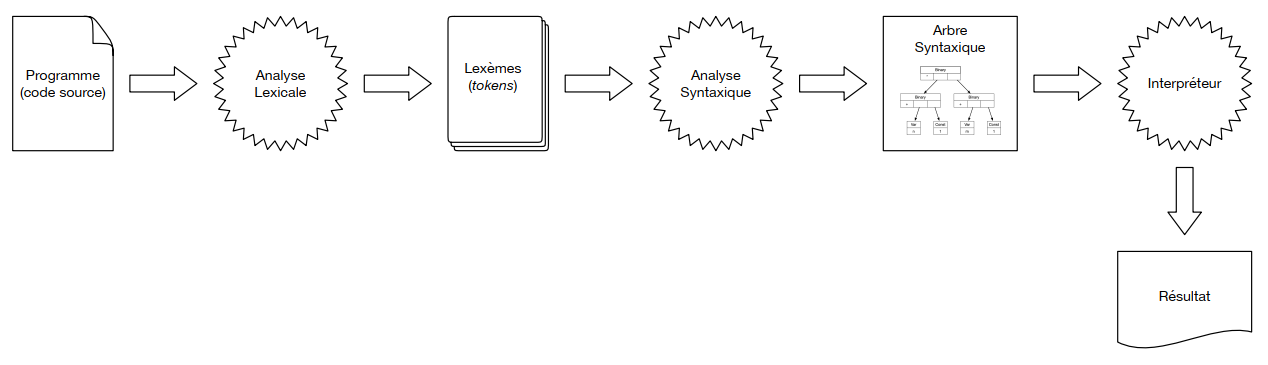
\includegraphics[width=12cm]{assets/figures/interpreter-flow.PNG}}
    \end{center}
    \caption[Analayse du code source]{\label{Analayse du code source} Analayse du code source}
\end{figure}

Dans notre cas, nous utiliserons seulement l'arbre et uniquement lorsque cela sera nécessaire.

\section{VS Code}
Il a été choisi, car il fait partie des éditeurs les plus populaires. C'est également l'éditeur que j'utilise le plus personnellement et donc je suis déjà familier de son environnement.
D'autres alternatives existent comme VIM et Atom pour ne citer qu'eux. Et chacun d'eux fournit également de quoi implémenter une extension.
C'est donc un choix personnel.

Visual Studio Code (ou VS Code) est un éditeur de code multi-plateforme, open source et gratuit.

Il est pensé pour être extensible (de L'UI à l'expérience utilisateur), presque tout peut être customisé et amélioré à travers de L'Extension API \cite{extension-api}.
On se focalisera sur le theming, les fonctionnalités de langages, la publication de l'extension et les tests.

VS Code fournit des documentations détaillées sur plein de sujets : étapes pour la création d'une extension, son déploiement continue ainsi que le support de langage en lui-même.
Il est aussi possible facilement de trouver des guides, ainsi que \href{https://github.com/microsoft/vscode-extension-samples}{des exemples de codes} concernant les extensions.
Il s'agit donc évidemment de la source principale des explications données dans ce document concernant ce qui touche à cet éditeur.
La communauté est aussi très active (stack overlow, gitter, issue github, etc.).

Le code source de VS Code de Microsoft est open source, sous licence MIT permissive.
Il a été écrit en TypeScript et JavaScript. Une extension peut être également écrite dans ces deux langages.
Nous choisirons le TypeScript car VS Code recommande ce langage. Mais certaines composantes externes (langage server) peuvent être écrites dans n'importe quel langage. Tant qu'elles fournissent l'API adéquate pour communiquer.

Un éditeur de code est un logiciel destiné à la création et l'édition de fichiers textes.
Contrairement à un IDE (Environnement de développement) qui permet en plus la compilation et le debuggage de programme plus complexe.
Nous manipulerons des fichiers statiques par la nature même de UON qui est un langage de sérialisation.

\subsection{Extension Anatomy}
Il y a trois concepts cruciaux à comprendre pour réaliser une extension.

\begin{itemize}
    \item \textbf{Activation Events}: des événements à partir desquels l'extension devient active \cite{activation-events}.
    \item \textbf{Contribution Points}: des déclarations statiques qui sont faites dans l'Extension Manifest "package.json" pour étendre l'extension. Il s'agit d'un ensemble de déclarations JSON faites au travers du champ "contributes" \cite{contribution-points}.
    \item \textbf{VS Code API}: un ensemble d'API JavaScript que nous pouvons invoquer dans le code \cite{vs-code-api}.
\end{itemize}

En général, l'extension est une combinaison de plusieurs \emph{Contribution Point} et l'utilisation de l'API pour étendre les fonctionnalités de VS Code.

\subsubsection{Extension File Structure}\label{Extension File Structure}

La structure de base d'une extension est illustrée par la figure \ref{basic VS Code extension structure}.

% https://tex.stackexchange.com/questions/98703/framebox-and-subfigure-with-dirtree-package
\begin{figure}[H] % \begin{figure}[!h]
    \centering
    \framebox[\textwidth]{%
        \begin{minipage}{0.9\textwidth}
            \dirtree{%
                .1 ..
                .2 vscode.
                .3 launch.json     // Config for launching and debugging the extension.
                .3 tasks.json      // Config for build task that compiles TypeScript.
                .2 .gitignore.
                .2 README.md.
                .2 src.
                .3 extension.ts   // Extension source code.
                .2 tsconfig.json  // TypeScript configuration.
            }
        \end{minipage}
    }
    \caption[basic VS Code extension structure]{\label{basic VS Code extension structure} basic VS Code extension structure}
\end{figure}

\textbf{Extension Manifest} :
chaque extension doit contenir un fichier \emph{package.json}. En plus des champs propres à Node.js, on peut spécifier des scripts, dépendances de développement et des champs spécifiques à VS Code.

\textbf{Extension Entry File} :
il s'agit du fichier prinicipal de l'extension (Extension.js).
De base, il contient deux fonctions : \emph{activate} et \emph{deactivate}.
La fonction activate est exécutée à l'activation de notre extension par un \emph{Activation Event}. On initialisera ici notre extension.
La fonction \emph{deactivate} est exécutée lorsque l'application devient inactive et sert principalement à nettoyer le code avant la désactivation de l'extension

\textbf{Remarque} : le niveau de customisation est assez élevé. La seule limitation indiquée et qu'il n'est pas possible d'accéder au DOM de l'éditeur.

Nous avons donc vu les briques de bases pour la conception d'une extension. Mais cette base est suffisante pour commencer à travailler.

Si vous souhaitez vous renseigner d'avantages sur l'élaboration d'une extension vous pouvez consulter la page \href{https://code.visualstudio.com/api}{suivante}.
Concernant les fonctionnalités générales de l'éditeur VS Code vous pouvez consulter consulter \href{https://code.visualstudio.com/docs}{la documentation officielle}.

\section{Support de langage}
VS Code fournit la possibilité d'ajouter du support pour un nouveau langage de programmation au travers d'implémentation de fonctionnalités. Ces fonctionnalités peuvent être classées en deux catégories détaillées
dans dans les sections \hyperref[Declarative language features][Declarative language features] et \hyperref[Programmatic language features][Programmatic language features] ci-dessous.

\subsection{Declarative language features}\label{Declarative language features}
Elles ajoutent un support d'édition de texte de base pour un langage de programmation.
Par exemple, les éléments suivants :

\begin{itemize}
    \item syntax highlighting
    \item snippet completion
    \item bracket matching
    \item bracket autoclosing
    \item bracket autosurrounding
    \item comment toggling
    \item auto indentation
    \item folding (by markers)
\end{itemize}

Il s'agit de fonctionnalités implémentées à l'aide de fichier de configuration.

% TODO : faire ref à l'explication ci-dessus ?
Puis, elles doivent être enregistrées comme \emph{Contribute Point}.

\subsection{Programmatic language features}\label{Programmatic language features}
Il s'agit de fonctionnalité plus riche et plus complexe à mettre en place (p.ex : "Hovers", "Go to Definition", "diagnostic errors", "IntelliSense" \space et "CodeLens".
Il y a deux approches pour les implémenter que nous allons voir ci-dessous.

\subsubsection{VS Code API (Direct implementation)}
La première solution est d'utiliser \href{https://code.visualstudio.com/api/references/vscode-api#languages}{l'API de VS Code} pour les fonctionnalités de langage.
Cette API permet d'implémenter directement les fonctionnalités du langage.
% TODO : s'assurer que l'api vscode une implementation de LSP ?
% Comment faire la transition entre mon implémentationa avec celle d'un langage server

Beacoup de fonctionnalités se font en s'inscrivant à des providers depuis notre application.
L'éditeur de code fera ensuite les requêtes à ces providers lorsque cela sera nécessaire.

\subsection{Language server}

La seconde solution est de fournir nous-mêmes ces méthodes en respectant la spécifiation LSP \cite{lsp-specification} au travers d'un langage serveur.
Les avantages souvent mentionnés ce cette approche sont que le langage server peut être écrit avec le langage que l'on souhaite et
que cela permet aussi à d'autres éditeurs de texte compatibles avec le langage server d'utiliser ces fonctionnalités sans devoir les implémenter de nouveau.

Pour être utilisé sur VS Code, un langage server à deux parties :
\begin{itemize}
    \item \textbf{Un client} : c'est une extension écrite en Javascript ou Typescript qui à accès à tous les endpoints de VS Code.
    \item \textbf{Langage server} : un outil d'analyse linguistique fonctionnant dans un processus séparé.
\end{itemize}

\vspace{\parskip}

Le client et le serveur communiquent à l'aide du protocole LSP (pour "language server") dès que des informations devraient être fournies à l'éditeur.

L'implémentation d'un tel serveur peut être libre en respect avec la spécification, mais des implémentations existent déjà. Telle que \emph{LSP4} implémenté en Java ou \emph{VS Code-languageserver-node}
implémenté en Typescript qui n'est pas exclusivement réservé à VS Code comme son nom pourrait l'indiquer.

Un langage server peut être utilisé sur d'autre éditeur compatible mais le client devra être implémenté de nouveau pour chaque éditeur.
Cette approche est aussi plus complexe à implémenter.

\subsection{API vs LSP}\label{api vs lsp}

Le schéma suivant \ref{api vs lsp} montre la correspondance des méthodes entre la première et seconde approche.

Cette liste est non exhaustive, mais permet de montrer l'équivalence des deux solutions.

\begin{figure}[!ht]
    \begin{center}
        \frame{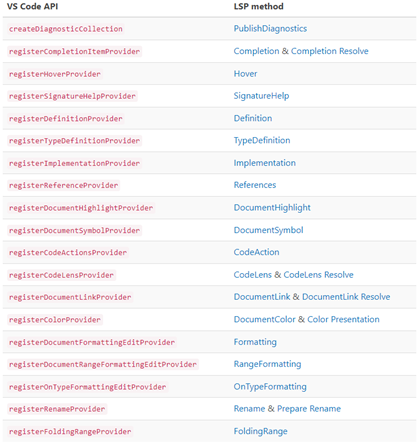
\includegraphics[width=8cm]{assets/figures/api-vscode.png}}
    \end{center}
    \caption[API vs LSP]{\label{api vs lsp} VS Code API vs LSP method}
\end{figure}

\subsection{Fault tolerant Parser}
Pour fournir des fonctionnalités de langue, un point souvent mentionnée est l'utilisation d'un parser.
Car l'arbre généré par celui-ci contient des informations concernant la structure du document utiles pour certaines fonctionnalités.

Des outils permettant la génération d'un parser existent à partir d'une grammaire et seront prévilégiés.

Cependant dans le cadre de son utilisation dans un éditeur ou IDE, il devrait être "fault tolerant".
Car la plupart du temps, le code dans l'éditeur est incomplet et syntaxiquement incorrect.
Mais l'on s'attend tout de même que certaines fonctionnalités continuent à fonctionner (ex : la outline view).

Le parseur doit donc pouvoir générer au mieux un parse tree qui à du sens depuis du code erroné.

On pourrait également se demander s'il est possible de se passer d'une telle strucutre et de n'utiliser à la place uniquement des expression régulières.
Cependant un problème majeur survient rapidement si on choisit cette approche, la récursivité devient extrèment difficle à traiter. \cite{antlr-mega-tutorial}

%"you cannot find a (regular) expression inside another one, unless you code it by hand for each level. Something that quickly became unmaintainable."
%Example : % TODO

\section{Choix technologiques}
Nous allons maintenant mentionner les technologies et approches choisies et expliquer les raisons.

\subsection{Direct implementation}
L'implémentation d'un langage serveur n'étant pas une priorité et pour se concentrer sur la réalisation des fonctionnalités, la solution de contacter directement l'API de VS Code a été privilégiée.
Si le temps le permet, toute la logique du code concernant les fonctionnalités riches\ref{Programmatic language features} pourrait être déplacée dans un langage server.

Beaucoup de possibilités existent comme mentionné au point \hyperref[api vs lsp]{API vs LSP}, les providers utilisés sont les suivants :
\begin{itemize}
    \item \textbf{registerCompletionItemProvider} : pour afficher des suggestions de complétions.
    \item \textbf{registerHoverProvider} : pour gérer le hover.
    \item \textbf{registerDocumentSymbolProvider} : pour afficher les éléments dans la Outline View.
\end{itemize}

\subsection{ANTLR}

\Gls{antlr} est un générateur de parser, il est actuellement dans sa quatrième version.
Il a été créé par Terence Parr à l'Université de San Francisco et est très utilisé, autant dans le monde académique que professionnel \cite{antlr}.

Le générateur prend en entré une grammaire, qui est un fichier décrivant formellement un langage. La grammaire d'ANTLR est décrite en utilisant la notation \Gls{ebnf}.
L'algorithme de parsing utilisé dans sa version la plus récente est le "Adaptive LL(*)" qui est décrit comme une amélioration de l'algorithme
"LL(*)" utilisé dans sa version précédente \cite{adaptive-ll}. L'algorithme "LL" est consiste à une analyse de l'input de gauche à droite et en construit une "Leftmost derivation" \cite{ll}.

ANTLR est composé de deux parties principales. Il y a l'outil en java qui permet de générer le lexer et le parseur, donc le code permettant de reconnaitre un langage comme mentionné à la section \ref{parsing}.
Ainsi que l'environnement d'exécution (runtime) qui permet leur exécution.

Il n'y a donc, seulement qu'un seul outil qui permet de générer le code dans les langages cibles. Et il est écrit en Java.

Pour pouvoir utiliser cet outil dans un environnement autre que Java, il est nécessaire de l'utiliser dans un runtime (environnement d'exécution) propre au langage souhaité.

Le runtime ainsi que les fichiers générés sont dans le même langage. La liste se trouve \href{https://github.com/antlr/antlr4/blob/master/doc/targets.md}{ici}.
Malheursement, le typscript n'en fait pas parti.

\subsubsection{antlr4ts}
Nous utiliserons donc antlr4ts, qui est un environnement d'exécution en typescript et donc parfaitement adapté pour VS Code.
Il a été conçu par Sam Harwell indépendamment de l'organisation ANTLR.

% https://github.com/tunnelvisionlabs/antlr4/blob/master/doc/targets.md

C'est un outil qui semble populaire est très utilisé.

L'initialisation de base est la suivante :

\begin{listing}[!ht]
    \begin{minted}{typescript}
        let inputStream = new ANTLRInputStream("var c = a + b()");
        let lexer = new ExprLexer(inputStream);
        let tokenStream = new CommonTokenStream(lexer);

        let parser = new ExprParser(tokenStream);
        let errorListener = new ErrorListener();
        parser.addErrorListener(errorListener);
        let tree = parser.expression();
    \end{minted}
    \caption{antlr-setup}
    \label{antlr-setup}
\end{listing}

\textbf{Remarque} :
Comme mentionné plus loin au chapitre \hyperref[grammar scope]{4}. Le précédent travail de Bachelor s'était concentré sur l'utilisation d'un parseur généré depuis une grammaire Lark.
L'implémentation de son parser n'a pas été privilégiée, car il aurait été nécessaire de créer l'infrastructure permettant de l'utiliser.
Et antlr4ts semble être un choix plus naturel dans un environnement VS Code.

\subsubsection{ATN}

La version 4 de ANTLR a comme avantage sur son ancienne version (ANTLR3) d'avoir la structure de la grammaire directement disponible dans le parser via
un mécanisme de machine à état \Gls{atn}.

Ci-dessous est illustré l'ATN d'une séquence en UON :

\begin{figure}[!ht]
    \begin{center}
        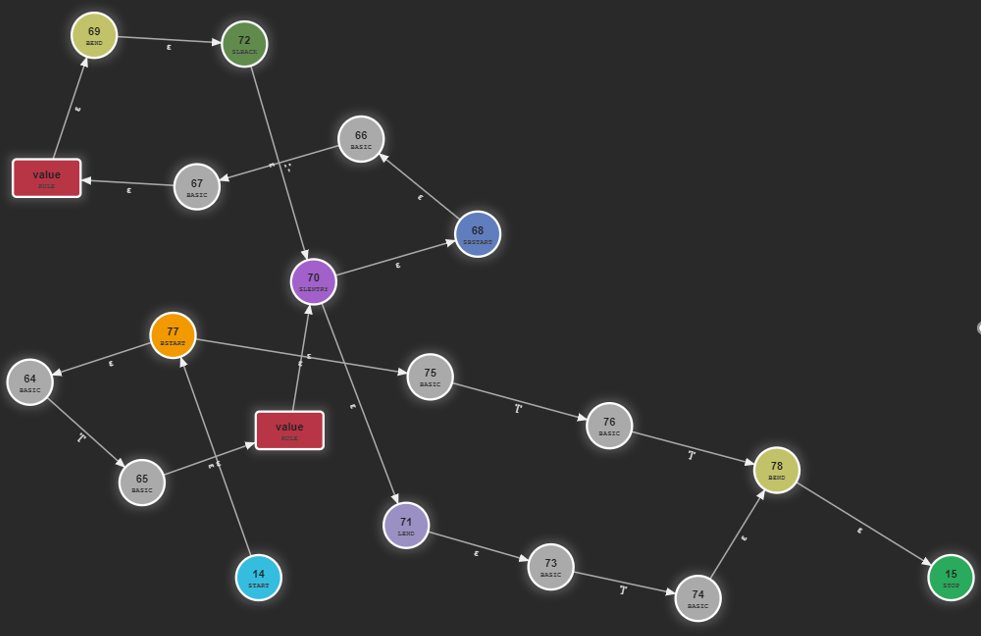
\includegraphics[width=12cm]{assets/figures/seq_ATN.png}
    \end{center}
    \caption[ATN d'une séquence]{\label{seq_ATN} ATN d'une séquence}
\end{figure}

\subsubsection{Gestion des erreurs}

%citation ?
ANTLR est capable de signaler des erreurs et se rétablir d'erreurs plus graves qui pourraient faire échouer le processus de parsing.
ANTLR définit l'interface \emph{ANTLRErrorStrategy} pour résoudre ce problème.
Elle sert à définir une stratégie concernant les erreurs rencontrées.

On peut distinguer trois types d'erreurs \cite{ANTLRErrorStrategy} :
\begin{itemize}
    \item L'analyseur syntaxique n'a pas pu déterminer le chemin à prendre dans l' ATN (aucune des alternatives disponibles ne pouvait correspondre).
    \item L'input actuel ne correspond pas ce que nous attendons.
    \item Un prédicat évalué comme faux
\end{itemize}


Par défaut c'est l'implémentation \emph{DefaultErrorStrategy} qui est appliquée et qui consiste à supprimer un token qui poserait problème ou en rajouter un s'il manquerait, avant de
se resynchronisation à l'ATN et de continuer le parsing.

Cette resynchronisation permet de continuer dans la règle courante que traverse le parser.

S'il ANTLR n'a pas pu se rétablir et qu'il a encore des erreurs, il va consommer tout les tokens qui suit celui qui a posé problème.
Puis, ce mécanisme s'arrêtera quand il réussira à trouver un token qui lui permettra de quitter la règle de parser courante sans la valider, mais permettant de continuer le processus de parsing.
Au pire des cas il s'agira d'un token de retour à la ligne \Gls{eof}.

C'est grâce à ce mécanisme qui fait que si nous utilisons le \emph{DefaultErrorStrategy} nous obtiendrons un parse tree dans tous les cas.

Malheursement, je n'ai pas pu explorer plus en profondeur ce mécanisme complexe de resynchronisation.
Cela pourrait se révéler intéressant pour tolérer plus d'erreurs au lieu d'une seul pour l'instant.


%https://medium.com/pragmatic-programmers/altering-antlrs-error-handling-strategy-80ce7d046730
%* The default implementation resynchronizes the parser by consuming tokens
%* until we find one in the resynchronization set--loosely the set of tokens
%* that can follow the current rule

%https://www.antlr.org/api/Java/org/antlr/v4/runtime/DefaultErrorStrategy.html
%https://pub.dev/documentation/antlr4/latest/antlr4/DefaultErrorStrategy-class.html

%https://stackoverflow.com/questions/18550031/how-to-control-error-handling-and-synchronization-in-antlr-4-c-sharp/18553706#18553706
%https://github.com/antlr/antlr4/blob/master/runtime/Java/src/org/antlr/v4/runtime/DefaultErrorStrategy.java


% https://stackoverflow.com/questions/25467627/how-to-continue-parsing-after-an-error-in-antlr-4-4
%Antlr 4's parser error strategy is to drop tokens from the input until it can detect a sane state and then
% it continues parsing. Looking at your example, while trying to recover maybe it never reaches a sane state before EOF.

%https://pub.dev/documentation/antlr4/latest/antlr4/DefaultErrorStrategy-class.html


%% UON se veut ête moins ambigue que ces alternatives pour l'utilisateur\dots
\section{UON}
UON est essentiellement un langage de sérialisation qui est un superset de JSON et un superset partiel de YAML.
Il cherche à regrouper les meilleures caractéristiques de ces formats de sérialisation en un seul format.
Il fournit également des fonctionnalités supplémentaires utiles pour augmenter l'interopérabilité entre différents types de dispositifs, valider les données ainsi que pour diminuer le payload.

Nous allons voir ci-dessous un aperçu général de ce langage.

\subsection{Format de sérialisation}

Lorsqu'on sérialise des données, elles se retrouvent soit sous forme binaire ou soit textuelle.
Ce projet se focalisera naturellement uniquement sur le format textuel, car c'est le seul format, humainement interprétable, que l'on manipulera dans un éditeur.
Le rôle d'un format de sérialisation et de pouvoir représenter des données sous une autre forme pour être ensuite manipulé.

Un éditeur ne manipulant qu'un fichier statique, les étapes de sérialisation et désérialisation ne se feront pas à notre niveau.
Pour pouvoir profiter de ces fonctionnalités, cela nécessite d'avoir un environnement de programmation (ex : Python).

% TODO : Sérialisation
% TODO : Desérialisation

% TODO : Parler des similutes différences
%\subsection{JSON}
%\subsection{YAML}
%\subsection{XML}

\subsection{Pourquoi ?}
Son rôle est d'être utilisé dans l'industrie 4.0. Plus particulièrement dans la communication m2m (machine to machine) ainsi que pour l'IoT (Internet of Things).
Ces communications nécessitent souvent de communiquer entre de petits appareils dont la puissance de calcul est très limitée.
La perspective de disposer d'un protocole de communication applicatif à la fois interopérable et adaptée aux échanges à faible puissance est très appréciable.
Parce que % TODO

\subsection{Communication}
Lorsque deux appareils veulent échanger des informations, ils disposent de deux canaux de communication :
\begin{itemize}
    \item Un canal de communication en ligne utilisé pour la transmission des données de contenu (payload). Les données peuvent être représentées sous forme humaine et binaire.
    \item Un canal de communication contractuel utilisé pour l'accord sur la description des données (schema).
\end{itemize}

\vspace{\parskip}

À la figure \ref*{data-exchange}, on a à gauche deux dispositifs : un capteur de température à faible consommation
et une puissante passerelle domotique. Pour réduire la taille du payload, les deux dispositifs peuvent convenir d'un schéma qui décrit le format des données.

\begin{figure}[H]
    \begin{center}
        \frame{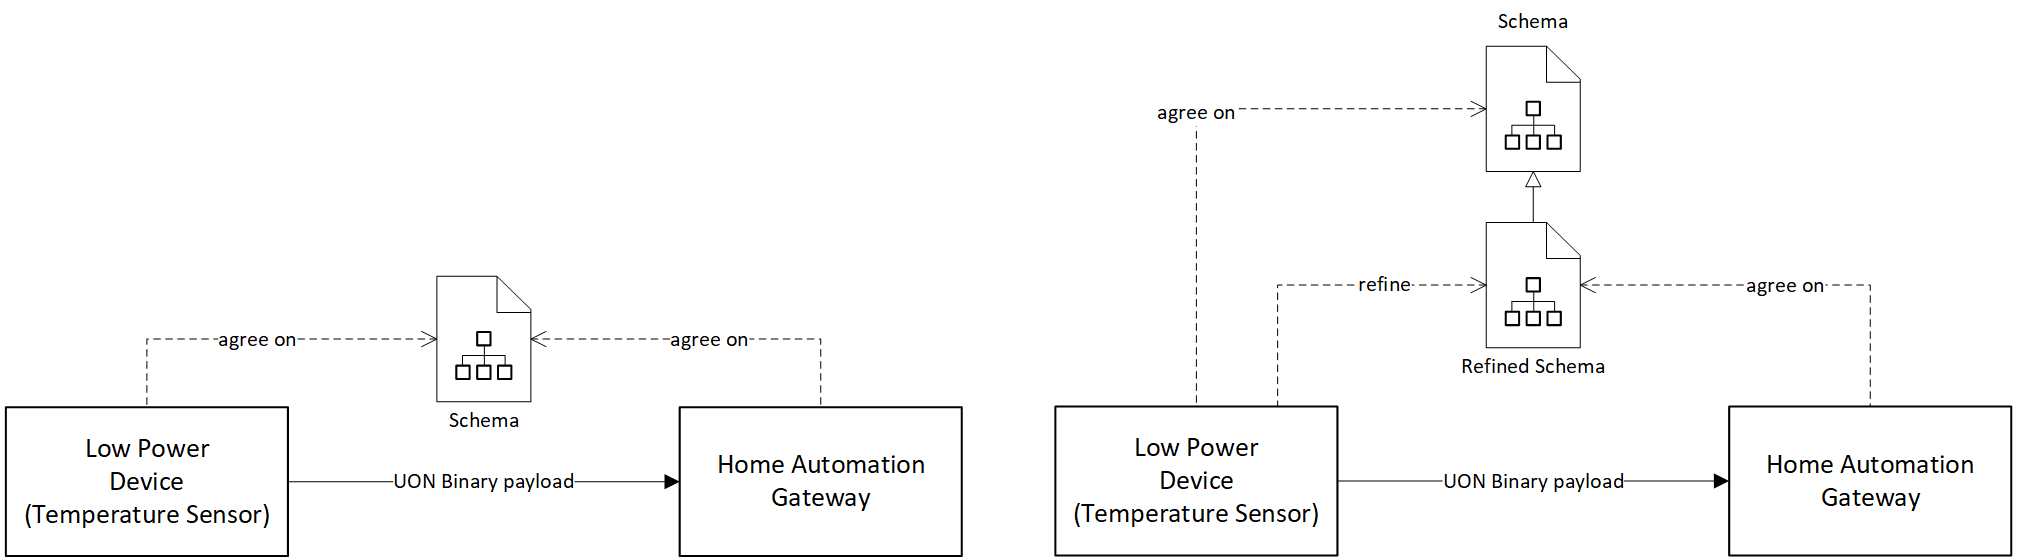
\includegraphics[width=15cm]{assets/figures/data-exchange.png}}
    \end{center}
    \caption[UON data exchange]{\label{data-exchange}UON data exchange}
\end{figure}

À droite on affine le schéma. Pour réduire davantage les données transmises.
Par exemple, en disant que la température exprimée avec un nombre est maintenant une valeur non signée de huit bits exprimée en degrés Celsius.

\subsection{Design}
UON est complètement conforme avec JSON et partiellement avec YAML.

Il peut être décomposé au travers de 4 niveaux de complexités :
\begin{itemize}
    \item \textbf{UON:0} est entièrement compatible avec JSON en ce qui concerne le RFC8259.
    \item \textbf{UON:1} est partiellement conforme à YAML.
    \item \textbf{UON:2} fournit des propriétés de type, la coercition et les chaînes de caractères multilignes.
    \item \textbf{UON:3} offre des types et des références riches.
\end{itemize}

\subsection{Types}
Chaque élément est composé d'un type. Et chacun de ces types peut avoir des propriétés.
3 types de propriétés existent :
\begin{itemize}
    \item \textbf{Presentation properties} : elles influencent la présentation d'une valeur.
    \item \textbf{Validation propeties} : elles sont utilisées pour valider, contraindre et décrire un fichier UON.
    \item \textbf{Application properties} : elles ne peuvent être lues que depuis UON en utilisant le type !prop. Elles sont accessibles depuis l'application (Python, JavaScript, etc.). Elles sont utilisées pour générer un fichier sérialisé (binaire, ou UON), mais elles ne sont jamais explicitement transmises.
\end{itemize}

\subsection{Validation}
Dans de telles communications, la validation des données transmises entre des machines dont la puissance de calcul est très limitée est un atout majeur.
Une des propriétés uniques de UON est l'usage de schéma directement intégré dans le langage.

% TODO : Lister les différentes formes de schéma de validation

\subsection{Liens}
Si vous souhaitez vous renseigner d'avantages, la spécification complète du projet se trouve sur cette \href{https://github.com/uon-language/specification/}{page}.
Et le dépôt du projet se trouve \href{https://github.com/uon-language/specification}{ici}.

% TODO : Datatypes ?

%% Résumé rapide de la grammaire initiale + dire qu'elle est relativement bonne et qu'on a pas modifier grand chose

%  Adaptation (passé de lark à antlr) (regex, espace différents, pas de librairie pour les indentations, ...)
%   YAML
%       Retirer dans un premiers temps le yaml
%   Indentation
%   Propriétés dans les types + de units

% On va pas tout spécifier mais relever certains point de la grammaire qui est pertinent
% Apercu de la grammaire plus en détail et exmple avec arbre + Examples
% Collection
% map
% seq
% clé-valeur
% clé IDENTIFIER
% nombbre

% Faire attention de faire le découpage pour la completion

\chapter{Scope de la grammaire}\label{grammar scope}
Pour pouvoir proposer du support pour un nouveau langage, il est nécessaire de savoir sur quoi celui-ci portera exactement.
Il est donc important de préciser sur quels éléments du langage nous nous focaliserons.

Une spécification d'UON existe, elle couvre énormément d'aspects. Cependant, tout n'est pas détaillé et donc des points sont sujetx à interprétation.
C'est un langage complexe et qui pourrait encore, être ammener à évoluer. Les propositions et les suggestions sont les bienvenues.

Heurseuement pour nous, une grammaire concrète avait déjà été écrite en Lark par l'ancien élève Stéphane Selim pour son travail de bachelor "Parser for a serialization language UON".
Son travail se trouve sur \href{https://github.com/uon-language/uon-parser}{ici}

Nous nous appuierons sur cette grammaire que nous convertirons en format ANTLR et ferons les modifications jugées nécessaires.

Les fonctionnalités se baseront sur celle-ci. Ceci dans le but de rester cohérents entre elles.
Nous ferons attention à son extensibilité et expliquerons les choix d'implémentations.
Elle sera complétée et améliorée après la mise en place des fonctionnalités attendues, si le temps le permet.

Cette grammaire se trouve décrite dans le fichier UON.g4 du projet.

\section{Résumé}
Pour commencer, il est nécessaire de préciser ce que permet cette grammaire initialement.
Nous utiliserons la grammaire qui a été adaptée dans le format d'ANTLR pour illustrer nos exemples.

% TODO EBNF ICI ? Type 2 de grammaire ?

\subsection{root value}

Un fichier UON peut contenir trois structures différentes.

\begin{lstlisting}[frame=single,caption={uon-root-value},label={uon-root-value}]
    uon: root_value;

    root_value: json_collection | schema;

    json_collection: json_map | json_seq;

    yaml_collection: yaml_map | yaml_seq;
\end{lstlisting}

\subsubsection{Collections}
La grammaire actuelle nous permet de définir des collections. Ces collections sont des mapping et séquences soit dans un format proche de json ou de yaml.

UON est par nature proche du format JSON. Mais UON étant "YAML compliant" à certain degré, mon prédécesseur avait jugé utile d'incorporer ce format
dans le langage. Cette structure a été reprise, mais expliquons à la section ? %TODO
les modifications nécessaires qui ont été apportées.

\textbf{Remarque} : par simplicité nous dirons qu'il s'agit du format "json" ou "yaml" lorsqu'on les mentionnera.

Ces collections peuvent être imbriqué par format, on ne peut pas avoir dans un fichier une collection en format json et yaml en même temps.

% TODO : exemple de map

\begin{lstlisting}[frame=single,caption={json-map},label={json-map}]
    {
        "name" ( description : a12 ) :  !str( comment : ok , optional: False) ok, # error with outline with simply 12
        age: !float !float128 !float32 +12.2 C,
        hobbys ( description : "what i like the most",  optional : false ) : !seq [
            "cinema", "sport", "etc..."],
        license  :  !bool  true,
        car:   !bool false,
        sensor ( optional : false , description : ok ) : !map {
            type: "temperature",
            parameters1: !seq [ 1, 2,3,4,5]}
    }
\end{lstlisting}

\begin{lstlisting}[frame=single,caption={yaml-map},label={yaml-map}]
ok :
    -  ok
    - !float32 12
    -
         - ok
ok2 : -23
\end{lstlisting}


% TODO : exemple de seq

\begin{lstlisting}[frame=single,caption={json-seq},label={json-seq}]
\dots
\end{lstlisting}


\begin{lstlisting}[frame=single,caption={yaml-seq},label={yaml-seq}]
\dots
\end{lstlisting}


\subsubsection{Schéma}
% TODO : schéma de validation externe \ref{}
On peut définir également un schéma de validation. Ce schéma doit se trouver dans un autre document que les deux structures ci-dessus.

Cette séparation permet d'éviter des ambiguïtés. On incite comme ça à l'utilisateur à séparer la logique entre différents fichiers.
Un schéma est un document qui décrit la spécification d'un nouveau type.

\begin{lstlisting}[frame=single,caption={yaml-seq},label={yaml-seq}]
    \dots
\end{lstlisting}

\subsection{Valeurs}

\subsubsection{Types}
Les terminaux peuvent être des string, des booleans ou des nombres.

\subsubsection{Propriétés}
Les clés des mapping des propriétés peuvent posséder des propriétés de présentation.
Les types dans un schéma de validation peuvent posséder des propriétés de validation.

\section{Modification}

%Les valeur des clé-valeurs peuvent être null mnt
%les types peuvent avoir des propriétés dans le payload
%quelques unités ont été rajouté

% TODO
Uon est un langage comprenant plusieurs composantes est particularités qui ne peuvent pas toutes être traité dans un simple éditeur de texte. (ex : cohercien)
%

Nous allons garder presque la même structure, car cette grammaire regroupe déjà des éléments importants du langage UON.
Cependant quelques points concernant la structure générale ont été modifiés.

Pour commencer il a fallu convertir la grammaire dans à la main car aucun convertisseur n’existe. Heursement ANTLR et Lark se basent sur une notation EBNF.
Ce qui fait que la structure de la grammaire reste relativement semblable.

Le seul point de divergence a été sur l'utilisation d'expressions régulières car la syntaxe de celle-ci varie légèrement. Et sur la gestion de l'indentation expliquée % ici todo

Concernant la structure d'un fichier de grammaire ANTLR .g4 il y a quelques subtilités à connaitre :

Le fichier doit comporter le même nom que la règle de départ. %UON.g4 -> uon

Les règles de lexer définissent comment une chaine de texte doit être tokenifier. Elles doivent être écrites en majuscule !
Les règles de parser définissent comment une suite de tokens sera intérprétée. Elles doivent être écrites en miniscule !

% \textbf{Attention} : Utiliser des majuscules pour une règle, correspond à définir un "Lexer rule" et utiliser des minuscules à un  "Parser rule".

%Par défaut un fichier de grammaire peut contenir des règles de lexer et de parser. Mais l'on peut les séparer pour améliorer la visibilié.

%On peut ignorer des tokens.

%fragement

%WS: [ \n\r\t] -> channel(HIDDEN);

%LINE_COMMENT: '#' ~[\r\n]* -> skip;

\subsection{YAML}
%TODO : permet
La grammaire permettait deux notations différentes pour les collections : une proche de json et l'autre de yaml.

%Car UON est un superset de JSON et un set partiel de yaml.
%La spécification indique bien que UON doit être compatible avec yaml 1.2 sans toutefois mention explicitement tous les points
% TODO

% Il a été décidé au milieu du projet, de se focaliser d'abord sur le format proche de JSON, et de revenir sur cet aspect cette phase réalisé.
Il a été décidé au milieu du projet, de se focaliser d'abord sur le format proche de JSON, et de revenir sur cet aspect si le temps le permet.
Car la notation en YAML pose quelques difficultés. % posait
En JSON les retours à la ligne et indentations ne sont pas nécessaires à la compréhension du langage, contrairement à YAML.
Nous expliquons dans le chapitre suivant il faudrait faire pour cohabiter ces deux formats avec ANTLR. % nous avons fait

\subsubsection{L'indentation}

% TODO : tsconfig.json
% TODO : stratégie switch
% TODO : changement minus

Contrairement au parser lark, la gestion des indentations n'est pas gérée automatiquement à l'aide d'une librairie externe.
Ce mécanisme doit malheureusement être traité par nos soins.

La grande modularité d'ANTLR est un avantage, mais peut se révéler très contraignante pour ce genre de tâches.

Mais avant de résoudre ce problème, il est nécessaire de rappeler que notre grammaire n'est pas uniforme concernant la gestion des retours à la ligne. 

Et c'est là où se trouve la vraie problématique.

En effet, UON peut être écrit sous une forme proche de JSON ou de YAML. Le premier ne tient pas compte des indentations contrairement à la seconde.

Et la gestion des indentations nécessite de prendre en compte les retours à la ligne. % TODO newline regex

Il y a donc trois solutions qui ont été envisagées.

La première est de rajouter des tokens de retour ou il serait jugé bon de les avoir dans la grammaire, et de les rendres optionnels.
Mais ce n'est pas très propre et on risque d'en placer énormément.

Le deuxième serait d'ignorer tout simplement les erreurs.  C'est-à-dire que si on à un token de retour à la ligne qui ne devrait pas être là, alors l'ignorer tout simplement.
On pourrait penser ce mécanisme simple se révélerait efficace. Cependant je n'ai malheureusement pas réussi à faire que le moteur de complétion c3
puisse ignorer ces erreurs.

La troisième solution trouvée et celle actuellement utilisée. Elle consiste à prendre en compte uniquement les retours à la ligne si le lexer à détecter les tokens initiaux
nous permettant de savoir nous avons à faire à une construction proche du JSON ou du YAML et donc savoir si les retours à la ligne doivent être pris en compte ou non.

Par exemple, tester si le premier token est un token de type MINUS ("-"). Si c'est le cas, on peut déduire qu'il s'agira d'une séquence en format YAML.

Dès lors que les retours à la ligne existent, nous pouvons maintenant placer les tokens INDENT et DEDENT depuis le lexer
pour pouvoir gérer les imbrications correctement.

Pour ce faire, à chaque fois qu'un espace qu'un retour à la ligne est détecté par le lexer, nous prenons compte de la taille de l'espacement qu'il contient ("\\r\\n    ")
Cet espacement nous permettra de savoir si l'on doit rajouter des INDENT ou DEDENT.

Le code permettant ce mécanisme peut être placé dans le fichier grammaire, en le plaçant dans le block \emph{lexer:@member{}}.
Lors de la génération, le code est placé dans le lexer.

Cependant lors de la génération les imports seront manquants, il est nécessaire d'aller les rajouter manuellement.

%Le code se trouvant sur le dépot suivant à été fortement utile : https://github.com/umaranis/FastYaml

% TODO : manque la partie avec le switch si on skip ou non les espaces utiles pour créer les tokens indent ou dendent

Il est maintenant possible d'avoir par exemple la règle suivante :

\begin{lstlisting}[frame=single,caption={generator-code},label={generator-code}]
    yaml_seq : INDENT (SEQUENCE_TYPE)? seq_item+ DEDENT;
\end{lstlisting}

\subsubsection{Minus}
\begin{lstlisting}[frame=single,caption={uon-number},label={uon-number}]
NUMBER:
	(('+'|'-')? INT ('.' [0-9]*)? EXP?) // +1.e2, 1234, 1234.5
	| '.' [0-9]+ EXP? // -.2e3
	| (('+'|'-')? '0' [xX] HEX+) // 0x12345678
	| (('+'|'-')? '0' [oO] HEX+) ; // 0o12345678

NUMERIC_LITERAL: 'inf' | 'nan' | '-inf' | '-nan' | '+inf' | '+nan';
\end{lstlisting}

Le caractère "-" étant utilisé pour définir une séquence en format yaml.
Il a fallu forcer le caractère directement dans l'expression régulière définissant un nombre.

\textbf{Remarque} : cette solution n'est pas optimale, car si on modifie la grammaire il faudra modifier ce code.

\subsection{String}

\begin{lstlisting}[frame=single,caption={uon-string},label={uon-string}]
    string :
	literal
	| QUOTED_STRING
	| UNQUOTED_STRING;
\end{lstlisting}

Une valeur textuelle peut soit être entre guillemets ou non.

C'est donc aussi le cas pour la clé d'une map.

Cela se rapproche par exemple, un peu plus de ce que fait JSON5 par exemple. % TODO lien
Aussi cela permet d'avoir des clés qui peuvent contenir exactement ce que l'on veut.
Car encapsuler entre des caractères spécifiques, il n'y a pas d'ambiguïtés possibles. Alors que sans on est contraint de limiter la forme de la clé.

Par contre un cas spécial a dû être traité. Si l'on veut pouvoir utiliser directement un mot sans guillemet, mais qu'il existe dans la grammaire.
Il faut ajouter ce cas, c'est pourquoi nous avons la règle de parser "literal" pour pouvoir utiliser un de ces tokens comme string.

\begin{lstlisting}[frame=single]
    {
        temperature : 10 C
    }
\end{lstlisting}

\begin{figure}[!h]
    \begin{center}
        \frame{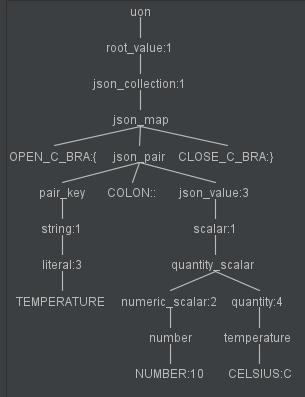
\includegraphics[width=8cm]{assets/figures/literal-key-uon.PNG}}
    \end{center}
    \caption[literal-key-uon]{\label{literal-key-uon}literal-key-uon}
\end{figure}

Sur le schéma \ref*{literal-key-uon} On voit que la clé et bien un token de type \emph{literal}.
Ce token \emph{temperature} existe comme token car c'est une valeur utilisée comme quantité, mais si on ne précise pas explicitement que l'on souhaite avoir cette valeur
comme possible clé alors on aura une erreur si on ne le précise pas \dots % TODO

\subsubsection{Unquoted}
%% TODO

\begin{lstlisting}[frame=single,caption={unquoted},label={unquoted}]
    UNQUOTED_STRING: IDENTIFIER+;

    IDENTIFIER
        : [\p{L}]    // matches a single code point in the category "letter"
        | [\p{M}]    // a character intended to be combined with another character (e.g. accents, umlauts, enclosing boxes, etc.)
        | [\p{N}]    // matches any kind of numeric character in any script.
        | [\p{Pc}]   //  punctuation character such as an underscore that connects words.
        | '!';
\end{lstlisting}


\subsubsection{Quoted}

%% TODO
\begin{lstlisting}[frame=single,caption={quoted},label={quoted}]
    QUOTED_STRING:
    '"' DOUBLE_QUOTE_CHAR* '"'
    | '"''"''"' DOUBLE_QUOTE_CHAR* '"''"''"'
    | '\'' SINGLE_QUOTE_CHAR* '\'';

    fragment DOUBLE_QUOTE_CHAR: ~["\\\r\n];

    fragment MULTILINE_QUOTE_CHAR: ~[];

    fragment SINGLE_QUOTE_CHAR: ~['\\\r\n];
\end{lstlisting}

N'importe quelle caractère peut se trouver

%% TODO : Multiline ? ne pas tolérer les espaces dans la clé mais dans le texte

\subsection{Propriétés, unités et nombres}

Des propriétés de présentation ont été rajoutées en reprenant les constructions utilisées pour définir des propriétés pour les clés ainsi que de validation.

% "_" dans le caption cause des erreurs !!!
\begin{lstlisting}[frame=single,caption={types properties},label={types_properties}]
    types_properties: OPEN_PAR (types_propertie (COMMA types_propertie)*)? CLOSE_PAR;
    types_propertie: comment | description | optional;
    comment: COMMENT COLON string;

    \dots

    string_scalar: (STR_TYPE (types_properties)?)? string;
\end{lstlisting}

number, bolean, null, string(literal, unquoted et quoted),
literal : tous les token utilisé déjà ailleurs mais qu'on voudrait avoir dans les clé par exmeple...

typs : string, nombre, boolean,

quantité et unités



\section{Debugging}

Il n'est pas simple de debugger une grammaire sans aucun outil ou seulement à l'aide d'un terminal, cela peut même se révéler extrêmement difficile.
Heursement pour nous, il existe une \href{https://plugins.jetbrains.com/plugin/7358-antlr-v4}{extension} sur intellij qui nous permet de visualiser en temps réel, le parse tree du texte que l'on est en train de saisir.

% TODO : Figure d'intelj en action

% Les figures représentants les arbres se baseront sur ce plugin ...


\chapter{Implémentation}
Dans ce chapitre, nous allons explorer les aspects techniques concernant l'implémentation de fonctionnalités. Nous allons voir également plus en détail les outils utilisés ainsi que le déploiement de l'extension sur le marketplace.
Ce travail reflète uniquement mon approche personnelle sur la matière. Et ne devrait pas être considérée comme l'unique manière de procéder.

%TODO
%\section{Tolérance}
%Le parseur ne devrait uniquement controler la syntaxe. une bonne règle à se rappeler et que dans le doute il est préférable de laisser l'analyser syntaxique (parser) 
%Le document et controler la sémantique pour s'assurer que la règle a du sens

%"The parser should only check the syntax. So the rule of thumb is that when in doubt you 
%let the parser pass the content up to your program. Then, in your program, you check the semantics and make sure that the rule actually have a proper meaning."
% Citation !!! mégathread ?


\section{Code}

Par rapport à la figure %todo
les points suivants au été rajouté à la figure %todo

\textbf{Remarque} : Les "..." signifie qu'il y a des sous fichiers et/ou répertoire mais ont été ignoré pous ne pas surcharger
la figure.

\begin{figure}[!h]
    \centering
    \framebox[\textwidth]{%
        \begin{minipage}{0.9\textwidth}
            \dirtree{%
                .1 ..
                .2 github.
                .3 workflows.
                .4 pipeline.yml.
                .2 vscode.
                .3 launch.json.
                .3 tasks.json.
                .2 .gitignore.
                .2 README.md.
                .2 src.
                .3 completion.
                .4 completion.ts.
                .3 error.
                .4 ErrorListener.ts.
                .4 UonCompletionErrorStrategy.ts.
                .3 generated.
                .4 ....
                .3 grammar.
                .4 .antlr.
                .4 UON.g4.
                .3 outline.
                .4 UonASTVisitor.ts.
                .4 UONDocumentSymbolProvider.ts.
                .3 test.
                .4 ....
                .3 extension.ts.
                .2 tsconfig.json.
            }
        \end{minipage}
    }
    \caption{UON VS Code extension structure}
\end{figure}

Le code de l'implémentation est disponible sur le dépôt public \href{https://github.com/vitorva/vscode-uon}{suivant}.

\textbf{Remarque} : L'implémentation détaillée dans ce rapport pourrait ne plus représenter l'état du dépôt, car ce projet est sujet à évoluer.

\section{Extension}
Nous allons voir maintenant, l'essentiel de la procédure pour créer et publier son extension.

La procédure détaillée se trouve \href{https://code.visualstudio.com/api/get-started/your-first-extension
}{ici}

\subsection{Génération de l'extension}

VS Code permet de générer un squelette (boilerplate) pour la réalisation d'une extension.
Pour ce faire il faut avoir Node.js et Git installés.

Ceci dans le but d'installer Yeoman et VS Code Extension Generator.

\href{https://yeoman.io/}{Yeoman} est un outil permettant de créer un générateur et de l'exécuter dans un environnement adapté.
\href{https://www.npmjs.com/package/generator-code}{VS Code Extension Generator} et le générateur implémenté par VS Code pour générer la structure de l'extension.

La commande pour l'installation est la suivante :

\begin{lstlisting}[frame=single,caption={generator-code},label={generator-code}]
npm install -g yo generator-code
\end{lstlisting}

Puis il suffit de lancer le générateur :

\begin{lstlisting}[frame=single]
yo code
\end{lstlisting}

Et de compléter ce qui est attendu dans le terminal pour créer notre extension.

\begin{figure}[!h]
    \begin{center}
        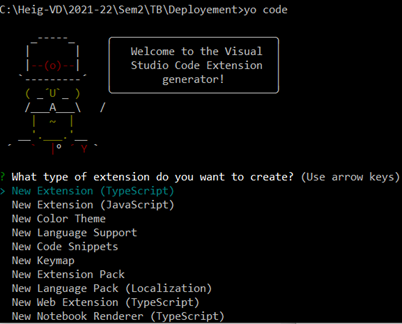
\includegraphics[width=8cm]{assets/figures/yo-code.png}
    \end{center}
    \caption[Yo Code generator]{\label{yo-code}Yo Code generator}
\end{figure}

Cela nous créera l'arborescence mentionnée précédemment au point \hyperref[Extension File Structure]{Extension File Structure}.

\subsection{Lancement de l'extension}
On peut lancer notre application en mode debug avec la touche F5. Cela va ouvrir une nouvelle fenêtre VS Code qui va contenir notre extension.

Par défaut, l'application générée vient avec du code permettant d'afficher un message de bienvenu. On l'affiche au travers du command pannel (CTRL + SHIFT + P). On peut s'assurer comme cela que l'implémentation de base fonctionne correctement.
On constate donc que par défaut, l'application doit être lancée au travers d'une commande, mais pour notre cas il sera plus intéressant que VS Code nous propose les fonctionnalités à l'ouverture d'un fichier UON.
Pour cela, il faut modifier \emph{l'activation events} dans le fichier package.json par :
\begin{lstlisting}[frame=single]
    "activateEvents" : [
	"onLanguage:uon"
    ]
\end{lstlisting}

\subsection{Déploiement sur le Marketplace}

% https://code.visualstudio.com/api/working-with-extensions/publishing-extension
% https://code.visualstudio.com/api/working-with-extensions/continuous-integration
% https://marketplace.visualstudio.com/manage/publishers/test2publish?noPrompt=true
% https://dev.azure.com/Stev03/_usersSettings/tokens

% delete publisher : https://stackoverflow.com/questions/54179509/how-do-you-delete-a-visual-studio-marketplace-publisher

% https://github.com/Microsoft/vscode-vsce/issues/249
% https://docs.npmjs.com/downloading-and-installing-packages-globally
% https://github.com/clangd/clangd/issues/159
% https://github.com/microsoft/vscode-vsce/issues/238

\textbf{Prérequis} : Posséder un compte Azure.

Il faut d'abord récupérer un Personal Access Token. Pour ce faire, il faut créer une \href{https://docs.microsoft.com/en-us/azure/devops/organizations/accounts/create-organization?view=azure-devops}{organisation}.
Puis, créer un access token avec ces paramètres :
\begin{figure}[!h]
    \begin{center}
        \frame{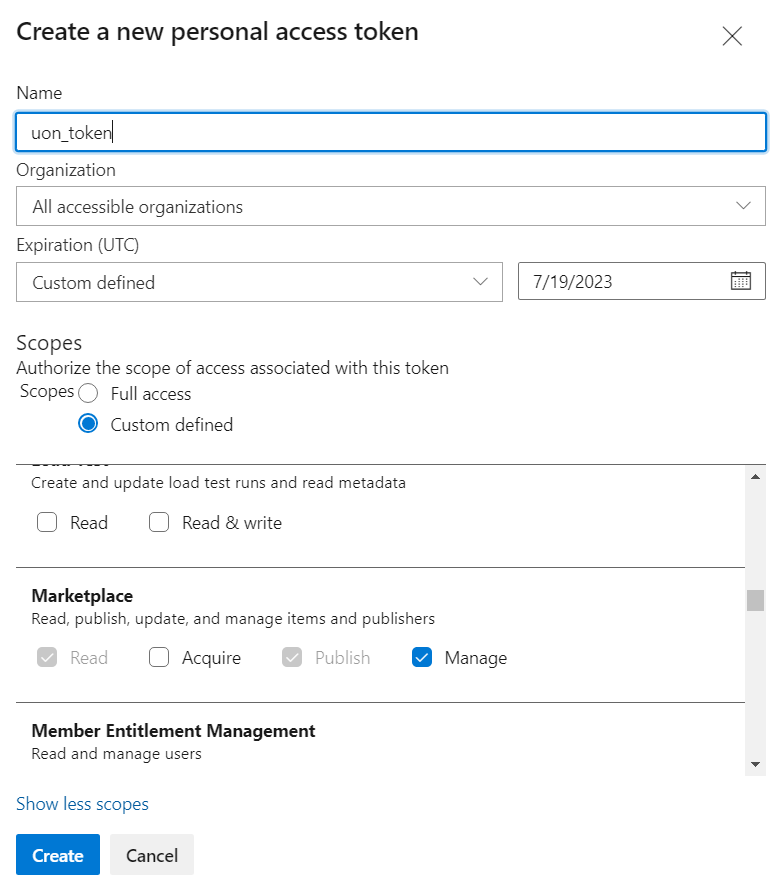
\includegraphics[width=8cm]{assets/figures/access-token.png}}
    \end{center}
    \caption[Access Token]{\label{access-token}Access Token}
\end{figure}

Ce token va nous permettre publier notre extension sur un Publisher. Celui-ci nous permettra de gérer notre extension en ligne.

Pour créer un publisher, il faut se connecter avec le même compte qui a créé l'organisation et le token ci-dessus via la \href{https://marketplace.visualstudio.com/manage/publishers/}{management page}.

Quand cela est fait, il faut ensuite ajouter la propriété "publisher" et saisir l'id de celui-ci dans le package.json de notre extension.

Puis finalement, il suffit dans un terminal de saisir les commandes suivantes :
\begin{lstlisting}[frame=single]
    vsce login [le nom du publisher]
    Vsce publish
\end{lstlisting}

\textbf{Remarque} : Attention au terminal utilisé. Dans mon cas, le terminal de node (git.bash) sur windows ne fonctionne pas lorsque des interactions avec le terminal sont nécessaires.

\begin{figure}[!h]
    \begin{center}
        \frame{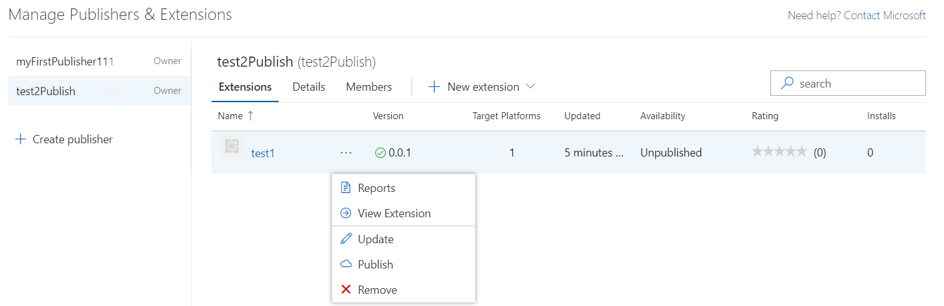
\includegraphics[width=12cm]{assets/figures/manage-publisher.png}}
    \end{center}
    \caption[Interface web pour manager l'extension]{\label{manage-publisher} Interface web pour manager l'extension}
\end{figure}

Il est ensuite facile de manager l'extension au travers de la page web.
L'extension apparaitra automatiquement dans le marketplace si elle est publiée.

\subsection{Intégration continue (CI)}

Comme le squelette de base de l'extension a été créé en utilisant le générateur Yeoman de VS Code, la structure pour écrire nos tests d'intégrations
existe déjà.
% citation : https://code.visualstudio.com/api/working-with-extensions/testing-extension

Il suffit de lancer la commande "npm run test" ou "yarn test" pour lancer les tests se trouvant dans le répertoire % TODO.

C'est l'api \href{https://mochajs.org/api/}{mocha} qui est utilisé pour ces tests.

Actuellement on teste de cette façon les fonctionnalités de la complétion et de l'outline view.

Concernant les tests pour la coloration syntaxique, le module \href{https://github.com/PanAeon/vscode-tmgrammar-test}{vscode-tmgrammar-test} a été choisi.
Car depuis mocha, on a pas moyen de le faire.

Nous avons donc quelques tests unitaires simples, mais qui permet toutefois de s'assurer qu'un changement ne vient pas modifier le comportement d'une manière inattendue.

Tous les tests se trouvent dans le dossier test à la racine du projet. % TODO lien avec l'arborescence

% TODO
\subsubsection{Autocomplétion}
On s'assure que les candidates de complétions attendues à un emplacement soient les bons selon une entrée de code.

\subsubsection{Syntax highlight}
créer un fichier .uon
faire un -snap
modifier le fichier snap et rajouter l'entête qui nous permet de définir que c'est un fichier tests
on peut maintenant le tester avec la commande : -test

% https://www.npmjs.com/package/vscode-tmgrammar-test?activeTab


\subsubsection{Outline view}
Un visiteur pour compter le nombre de noeuds attendus pour s'assurer qu'on soit bien passé par les noeuds

% Créer les construction à la main et comparer leur sorti textuelles

%REGEX
% utilisation d'outils en ligne : ex : https://regex101.com/
% référence officielle : https://www.regular-expressions.info/


\subsection{Deployement automatisé (CD)}

L'extension est actuellement automatiquement déployée lorsqu'une release sur la branche main est réalisée.
L'étape de mise en place est détaillée par VS Code à cet \href{https://code.visualstudio.com/api/working-with-extensions/continuous-integration#github-actions}{emplacement}.

Il s'agit d'une étape supplémentaire dans la pipeline après que les tests soient effectués.

Elle consiste à exécuter la commande vsce publish depuis notre package.json pour publier l'extension.

\href{https://www.npmjs.com/package/vsce}{vsce} est le gestionnaire d'extension de VS Code.

Il est nécessaire d'ajouter le token (PAT) comme secret dans notre dépôt github. %todo ref

\textbf{Remarque } : On ne peut déployer qu'une extension avec une version supérieure que la précédente. % TODO : automatisé ça ?


% TODO : maintenance
%Les explications permettant de reprendre le projet se trouve sur le Readme à la racine du repository
% Ne devrait pas faire parti de l'organisation du prof ?


\section{Génération du parser ANTLR}
\subsubsection{Grammaire}

Quand le fichier de grammaire est écrit, il suffit de lancer le code suivant :

\begin{lstlisting}[frame=single]
    antlr4ts -visitor path/to/MyGrammar.g4
\end{lstlisting}

Il nous génère ces fichiers :
\begin{itemize}
    \item UON.interp
    \item UON.tokens
    \item UONLexer.interp
    \item UONLexer.tokens
    \item UONLexer.ts
    \item UONParser.ts
\end{itemize}

\section{Syntax highlighting}

% Pour signaler à l'utilisateur que la saisie est tout de même incorrecte. On peut s'aider en parallèle de la coloration syntaxique.

La coloration syntaxique permet que chaque élément du texte soit affiché dans l'éditeur avec une coloration et un style en fonction de son type.
Il y a deux composantes principales. % Citation vscode ?
\begin{itemize}
    \item La tokenisation qui consiste à séparer le texte en une liste de token.
    \item La thémisation (Theming) qui permet d'attribuer à un token une couleur et un style.
\end{itemize}

%TODO : à changer
\begin{figure}[!h]
    \begin{center}
        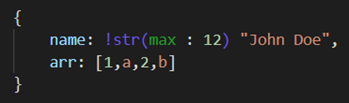
\includegraphics[width=10cm]{assets/figures/basic-uon.png}
    \end{center}
    \caption[code UON]{\label{basic-uon} Exemple basique en UON}
\end{figure}


VS code utilise Textmate grammars \cite{textmate-grammars} comme le moteur de tokénisation de la syntaxe.
Cette grammaire a été inventée par l'éditeur TextMate est a été adopté par de nombreux éditeurs et IDE.
Elle contient une liste structurée d'expressions régulières qui permet d'associer un scope
à un ou plusieurs tokens qui déclencherait l'activation d'une de ces expressions.

Nous définissons notre grammaire TextMate dans le fichier "uon.tmLanguage.json" qui se trouve dans le dossier "syntaxes" à la racine du projet.
Ce fichier doit être référencé à travers du point de contribution "grammar" dans le package.json.

% TODO : https://macromates.com/manual/en/language_grammars

%Le but de ce fichier en plus de permettre la coloration syntaxique, et qu'il permet également de rendre l'éditeur de texte "intelligent" quant au contexte dans lequel se trouve le caret.
%Cela permet d'avoir des comportements différents selon la situation (ex : Pas de bracket closing dans les commentaires).

\subsection{Scope}
Un scope défini le contexte d'un groupe de token et peut-être considéré comme son type.

Il s'agit d'un identifiant, c'est grâce au scope d'un token, qu'un fichier de thème peut attribuer une couleur avec un mécanisme de "clé-valeur".

TextMate liste une liste de scope commun que de nombreux thèmes ciblent déjà et recommande de les utiliser.
Ceci dans le but de permettre à notre langage d'être supporté le plus possible.
%% https://macromates.com/manual/en/language_grammars

Pour respecter au maximum les conventions attendues et s'assurer qu'une coloration automatique soit appliquée. La stratégie suivante a été adoptée : partir depuis un fichier de thème déjà créé (Thème dark par défaut sur VS Code). 
Et de réutiliser les scopes définis dans ce fichier.

Ce fichier se trouve sur le dépôt \href{https://github.com/microsoft/vscode/blob/main/extensions/theme-defaults/themes/dark_vs.json}{suivant}.
Mais peut être également généré depuis le contrôle panel (CTRL + SHIFT + P).

Ce procédé nous permet de profiter des thèmes de VS Code implémenté par défaut dans l'éditeur, par exemple les deux suivants :

\begin{figure}[!h]
    \begin{center}
        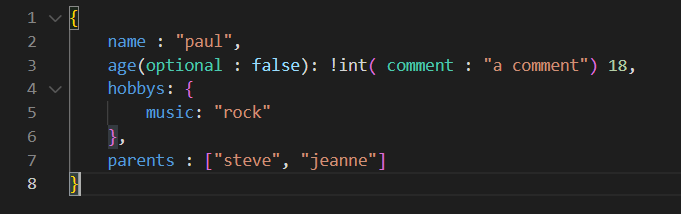
\includegraphics[width=10cm]{assets/figures/vscode-dark-theme.PNG}
    \end{center}
    \caption[vscode dark theme]{\label{vscode-dark-theme} vscode-dark-theme}
\end{figure}


\begin{figure}[!h]
    \begin{center}
        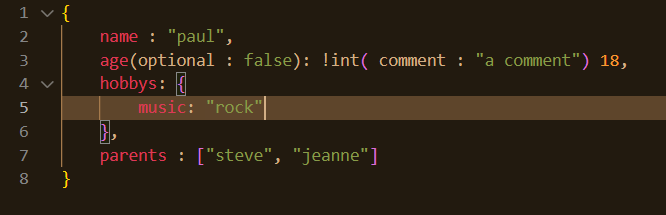
\includegraphics[width=10cm]{assets/figures/vscode-kimbi-dark-theme.PNG}
    \end{center}
    \caption[vscode kimbi dark theme]{\label{vscode-kimbi-dark-theme} vscode kimbi dark theme}
\end{figure}

\subsubsection{Example}
Prenons un exemple simple, le scope pour les nombres : "constant.numeric.uon"

On voit qu'il s'agit d'une suite d'identifiant.

La convention est d'avoir des mots clés séparés par un point pour spécifier chaque niveau de précision supplémentaire

Il est aussi possible d'avoir plusieurs scope pour un élément : "string.uon support.type.property-name.uon"

Les scopes sont séparés par un espace.
C'est celui le plus à droite qui l'emporte. Cela peut-être utile si l'on souhaite maximiser les chances qu'un thème nous fournisse une coloration.

% https://macromates.com/manual/en/scope_selectors

Les scopes sont souvent imbriqués et c'est le plus spécifique qui est utilisé pour le choix du thème.
Il est possible d'analyser notre code à l'aide du "Scope Inspector", qui est un outil disponible dans l'éditeur depuis le control panel,
pour visualiser la hiérarchie des scopes pour un token.

\begin{figure}[!h]
    \begin{center}
        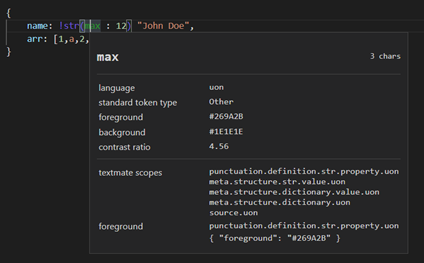
\includegraphics[width=10cm]{assets/figures/scope-inspector.png}
    \end{center}
    \caption[Scope inspector]{\label{basic-uon} Le scope inspector sur un exemple de code en UON}
\end{figure}

La section "textmate scopes" montre la liste des scopes utilisés pour le token qu'on séléctionne. Le scope le plus spécialisé se trouve au sommet.

La coloration syntaxique n'est pas considérée comme un "programmatic language feature" et donc n'est pas gérée par la spécification LSP et par l'API de VS Code non plus.
Une des raisons évoquées et que ce mécanisme doit être le plus rapide possible. Et que le faire directement depuis le client garantit une latence faible.
%citation d'un repo

\subsection{Fonctionnement}

Voici ci-dessous un exemple relativement simple, mais permettant de comprendre le mécanisme général utilisé dans notre fichier "uon.tmLanguage.json" :
\begin{lstlisting}[frame=single, caption={Textmate grammar},label={Textmate grammar}]
 1  {  scopeName = 'source.untitled';
 2     patterns = (
 3        {  name = 'keyword.control.untitled';
 4           match = '\b(if|while|for|return)\b';
 5        },
 6        {  name = 'string.quoted.double.untitled';
 7           begin = '"';
 8           end = '"';
 9           patterns = (
10              {  name = 'constant.character.escape.untitled';
11                 match = '\\.';
12              }
13           );
14        },
14     );
15  }
\end{lstlisting}
\textbf{"scopeName"} (ligne 1) : Scope racine du fichier

\textbf{"patterns"} (ligne 2) : C'est un tableau contenant les règles actuelles utilisées pour parser le document. Elles sont appliquées dans l'ordre.
Ces règles peuvent être directement écrites à cet emplacement, mais il est aussi possible de les définir dans le "repository". Puis de les inclure.

\textbf{"repository"} : Un dictionnaire (clé-valeur) de règles.

\textbf{"name"} : Nom d'un scope

On constate deux constructions possibles.
La première règle applique le scope à un élément qui déclenche le match.
La deuxième définit un délimiteur de début et de fin .

% TODO : pas clé
Les règles se trouvant dans la clé "patterns" suivante (à la ligne 12) seront appliquées aux éléments se trouvant à l'intérieur de ces délimiteurs.
On voit qu'il est donc possible d'imbriquer les règles.

\subsection{uon.tmLanguage}

%TODO


\subsubsection{Propriétés}

La coloration syntaxique doit refléter au mieux cette grammaire. Il y a donc une coloration spécifique pour les propriétés appartenant à un type.
Cela rend la coloration syntaxique fortement liée à la grammaire, mais on se rend compte d'un coup d'oeil si la propriété et correcte.

% TODO : propriétés pas définis

\subsection{Capture}

Il y a globalement deux manières pour appliquer un scope.

La première et de définir un caractère de départ et un autre de fin. Puis définir les patterns que l'on appliquera aux éléments se trouvant à l'intérieur.

% exemple : !str(comment : "mon premier commentaire")

Mais dans certains cas, il n'y a pas de délimiteur et on voudrait appliquer une coloration différente aux éléments qui composent le groupe de caractère qu'une expression régulière
a déclenché.

Il s'agit d'un nombre mais l'option "Capture" nous permet d'appliquer un scope au groupe de sélection.
Il n'est pas facile pour des expressions assez complexes de trouver ce nombre mais on peut s'aider du site \href{https://regex101.com/}{suivant}

\subsection{Semantic Highlight}

Un point important et qu'il ne faut pas confondre la coloration syntaxique avec ce que l'on nomme la coloration sémantique. Car il s'agit d'une couche que l'éditeur rajoute sur la précédente pour l'améliorer si nécessaire.
La tokénisation sémantique permet de fournir des informations supplémentaires sur les tokens en se basant sur une compréhension profonde du langage.
De manière à résoudre les symboles dans le contexte d'un projet.

Il s'agit donc d'obtenir des informations contextualisées afin fournir une coloration plus précise pour un token.

Par exemple avec du code Typescript :

\begin{figure}[!h]
    \begin{center}
        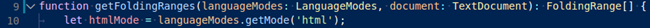
\includegraphics[width=15cm]{assets/figures/semantic-coloration-without.png}
    \end{center}
    \caption[Sans coloration sémantique]{\label{semantic-coloration-without} Sans coloration sémantique}
\end{figure}

\begin{figure}[!h]
    \begin{center}
        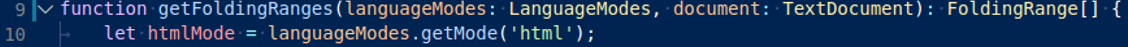
\includegraphics[width=15cm]{assets/figures/semantic-coloration-with.png}
    \end{center}
    \caption[Sans coloration sémantique ]{\label{semantic-coloration-with} Avec coloration sémantique }
\end{figure}

On voit à la ligne 10 que la colorisation de la fonction a changé et correspond maintenant à un paramètre d'une fonction.
Cela est donc intéressant pour des langages plus complexes dans leur nature qu'un langage de sérialisation. Une coloration syntaxe suffit amplement dans notre cas.
Car se baser sur la structure du document nous donne déjà toutes les informations nécessaires.

\section{Auto-completion}

% exemple de completion final

Cette fonctionnalité fait parti de ce qu'on appelle plus communément "IntelliSense" \cite{intelliSense} qui un terme général désignant diverses fonctions d'édition de code.

Le terme "auto-complétion" existe également sous d'autres appellations (ex : autocomplétion, complétion automatique, complétion, etc.).
L'intérêt est de proposer des suggestions de saisie au fur est à mesure que l'on écrit.

Il s'agit d'une fonctionnalité informatique permettant à l'utilisateur de limiter la quantité d'informations qu'il saisit avec son clavier
en se voyant proposer un complément qui pourrait convenir à la chaîne de caractères qu'il a commencé à taper.
% TODO : citation wikipedia

Le terme "suggestions" étant relativement vague. C'est ici où réside la subtilité. Cela va dépendre principalement du langage traité.

Car en JSON ou en YAML, l'auto complétion n'existe pas vraiment dû à leur nature même de ces langages de sérialisation.
Et contrairement à des langages de programmation. Il n'y a pas de mots clés, on ne peut pas définir de nom de fonction ni de classe.
On ne peut également pas définir de variables.

On n'aurait donc rien de base à proposer pour ces deux langages, sans utiliser une source d'infomation externe comme les "JSON-schéma".
À la limite, seules les clé ou valeur précédemment saisies peuvent éventuellement être reproposé mais cela est fait automatiquement sous VS Code
avec le type de complétion nommé "word based completion".
% https://stackoverflow.com/questions/54827043/how-to-disable-abc-suggestion-on-vs-code

Donc pour commencer, lorsqu'on implémente une telle fonctionnalité, il faut pouvoir répondre à quelques questions aux préalables.
Quelles sont les suggestions pertinentes à proposer ? Quand faudrait-il les proposer ?

Il est donc nécessaire d'analyser le langage UON et de voir ce qu'il est pertinent de proposer comme suggestion de complétion.

La syntaxe UON peut être exprimée par la figure \ref{syntax}.

\begin{figure}[!ht]
    \begin{center}
        \frame{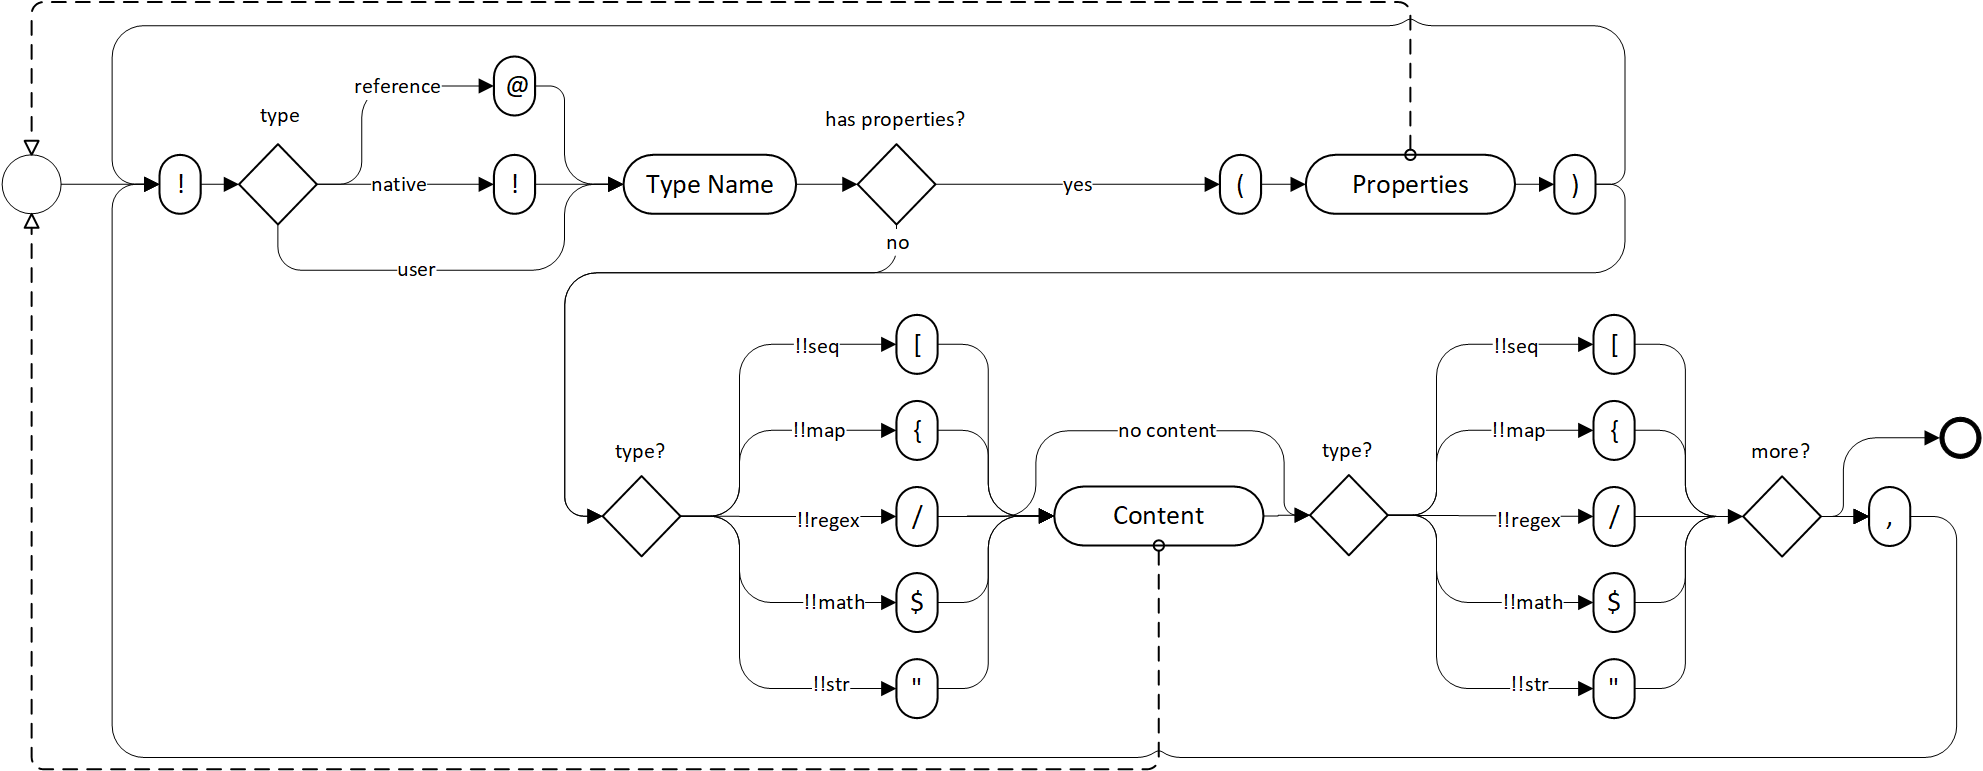
\includegraphics[width=12cm]{assets/figures/syntax.png}}
    \end{center}
    \caption[syntax]{\label{syntax} UON syntax}
\end{figure}

On y remarque des points extrêmement intéressants.

Toute valeur est un type, et un type peut avoir des propriétés associées.

Les suggestions de baseront donc sur les types et leurs propriétés.

\subsection{antlr4-c3}

Comme mentionné au début de ce document, une approche typique pour implémenter de la complétion est d'utiliser un parser du langage.

Mais en complément nous allons aussi utilisé \href{https://github.com/mike-lischke/antlr4-c3}{"antlr4-c3"} (également simplement nommé c3).

Avant il n'y a avait que des solutions personnelles. Cette librairie a pour objectif de fournir une implémentation commune.
Elle est disponible comme node module et est écrit en Typescript.

Elle a été conçue par \href{https://github.com/mike-lischke}{Mike Lischke}.

Cet outil est écrit en Typescript mais existe aussi en version \href{https://github.com/mike-lischke/antlr4-c3/tree/master/ports/java}{JAVA} et \href{https://github.com/mike-lischke/antlr4-c3/tree/master/ports/c%23}{C\#}.

Il s'agit d'un moteur de complétion pour les parsers basés sur ANTL4. Le moteur c3 est capable de fournir des candidats de complétions.
Nous utiliserons principalement ces candidats pour les suggestions proposées dans l'éditeur de code.

c'est un outil relativement puissant, qui nous simplifie grandement la tâche

% citation https://tomassetti.me/code-completion-with-antlr4-c3/
% Le moteur de complétion n'utlise pas le parse tree pour proposer des candidats, mais est il est quand même nécessaire de lancer l'exécution du parser (parser.uon()) pour remplir le stream de token (tokenStream).

% citation MEGA TUTO
Le moteur de complétion n'utilise pas le parse tree pour proposer des candidats. Mais l'exécution du parser est nécessaire pour remplir le token stream \ref{antlr-setup}.
Car le moteur s'appuyera sur ce flux de tokens et également du mécanisme de machine à état (ATN) d'ANTLR4 disponible dans le parser.

% citation
\textbf{Remarque} : Le résultat du parsing n'a pas besoin d'être correct. Il est possible de travailler avec du code incomplet ou malformé, ce qui est relativement fréquent dans un éditeur.

Pourquoi un tel moteur ?
Car connaitre tous les types de tokens qu'un utilisateur serait amené à saisir ne suffit pas. Pour que la complétion soit réellement intéressante, nous voudrions connaitre quelle règle de la grammaire pourrait être valide à une position donnée.
Et cet outil apporte une solution pratique est élégante pour résoudre ce cas.

Pour notre scénario, on voudra proposer des suggestions à la position du curseur, ce qui fait le code après celui-ci ne nous intéresse pas (dans le cadre actuel du langage).
On utilisera la position du curseur (caret). Pour uniquement traiter le code du début de l'éditeur jusqu'à la position du curseur.

Une utilité de prendre en compte ce qui se trouve après le curseur serait par exemple le cas de code SQL :

\begin{lstlisting}[frame=single]
SELECT | FROM USER // ("|" étant le curseur)
\end{lstlisting}

Dans ce scénario des suggestions liées à la table USER devrait être proposé et nécessiterait un traitement particulier.

Pour recevoir des candidats, il suffit d'avoir un environnement comme présenté par la figure \ref{antlr-setup}, d'installer le module npm \emph{antrl4ts} et
de donner au moteur, une instance du parser et un indice.

\begin{lstlisting}[frame=single] % TODO
    let core = new c3.CodeCompletionCore(parser);
    let candidates = core.collectCandidates(index);
\end{lstlisting}

L'explication pour trouver cet indice se trouve dans la section \hyperref[candidates]{\textbf{Candidats}}.
% \textbf{Remarque} : L'indice est calculé en se basant sur la taille totale du stream de token. (voir fichier completion.ts)

Cependant une contrainte pour que le moteur propose des candidats est qu'il est nécessaire que tout le code se trouvant avant le curseur soit correct.
Comme mentionné plus tard %TODO

Ce qui se trouve à la suite peut être erroné, car on ne n'en tient pas compte, comme mentionner ci-dessus.

Nous recevrons alors un objet de type \emph{CandidatesCollection}.

\begin{lstlisting}[frame=single]
    class CandidatesCollection {
        tokens: Map<number, TokenList>;
        rules: Map<number, RuleList>;
    }
\end{lstlisting}

Cette collection contient deux map.

\textbf{tokens} : fait le lien entre le prochain token possible et une liste contenant des tokens qui doit le suivre immédiatement, si elle existe.

Nous allons uniquement utiliser les clés de cette map pour proposer nos suggestions.

Car la liste n'est jamais utilisée actuellement, il n'y jamais deux tokens qui devrait se suivre obligatoirement dans la grammaire qui sont proposés par le moteur.

Par exemple pour obtenir une séquence de token comme dans l'exemple suivant :

\begin{lstlisting}
    !map {switch : |}
                   - !bool
                   - !bool true
\end{lstlisting}

Cela nécessiterait d'adapter la grammaire en conséquence pour que la valeur "true" soit le seul élément possible qui suit "!bool".

% TODO
% - parler de comment convertir ce symbole en token
% - c'est quoi la valeur concrètement : La valeur d'un token ou son nom ?


\textbf{rules} : fait le lien entre la règle du parser actuelle et la liste de règles utilisé pour arriver à ce stade.

Cette map nous permet de questionner la liste des symboles pour retourner des informations supplémentaires.

% TODO https://github.com/lark-parser/lark/issues/684

%Comment aurions nous du procéder sans un tel outil ?
%Il évidemment possible de le faire sans ce moteur.
%Un excellent article mentionne une telle implémentation aussi avec ANTLR ici.

%Cela rend bien entendu le travail plus conséquent.

\subsubsection{Symbol tables}

C'est un mécanisme puissant de c3 mais que nous n'allons pas exploiter,
car je n'ai pas trouvé d'usage dans le cadre du cahier des charges de ce projet et par manque de temps.
Cependant il reste intéressant de détailler brièvement son utilité pour d'éventuelles améliorations.

On pourrait penser qu'avoir à disposition un parser nous permettrait de récupérer toutes les informations nécessaires au travers d'un AST. % TODO AST abbréviation
Cependant ce n'est pas le cas pour la plupart des scénarios.
Nous pouvons savoir quels sont les tokens valide à un emplacement (ce qui est suffisant pour nous). Mais pour certains langages, des informations manquent.
Et c'est ce que la table de symboles essaye de résoudre.

Une table de symboles est une structure qui contient des informations complémentaires sur des symboles, cela peut s'agir de noms, leur scopes et d'autres caractéristiques.
Cependant, un langage de sérialisation est relativement moins complexe à gérer qu'un langage de programmation.
Nous n'avons par exemple pas à mémoriser des variables et leur visibilité au sein du code.

Mais il est mentionné dans la spécification qu'un schéma pourrait être défini au même niveau que le payload.
Avec ce scénario en tête, une table de symboles pourrait se révéler utile.

Car on pourrait se servir de ce schéma de validation qui spécifierait un nouveau type pour proposer de la complétion appropriée
lorsque l'on saisira ce type dans le payload. Typiquement des propriétés.

\subsection{Tokens ignorés}

Il est possible d'indiquer au moteur les tokens qu'il peut ignorer, pour ne pas les récupérer dans la liste des candidats fournis par le moteur.
Cela est nécessaire pour nous, car tous les tokens ne sont pas intéressant.

Les tokens peuvent être classé en deux catégories.

Ceux dans la valeur sont fixes
Ceux dans la valeur dépendent de la saisie d'un utilisateur au travers d'expression régulière.

La seconde n'est pas intéressante, car le moteur ne fera que retourner le nom du token ce qui est inutile.
La première catégorie, il faut aussi ignorer les tokens : parenthèse, accolades et les deux-points, car ce n'est pas vraiment pertinent.

\subsection{Gestion des erreurs }\label{error handle}

On aurait pu penser naïvement que le mécanisme avancé de récupération d'erreur \emph{Parser Error Recovery Strategy} permettrait également de rendre celui de la complétion aussi plus tolérant.
Mais ce mécanisme n'est utilisé que pour générer un parse tree, cela est donc inutile pour ce cas. % car se base sur TODO

Donc comme déjà mentionner, pour que le moteur puisse retourner des candidats, la syntaxe se trouvant avant la position du curseur doit être valide.
Car sinon on pourrait avoir dans le stream de token des éléments qui ne seront pas compris par le moteur et l'on n’obtiendra pas de candidats.

Une explication fournit par le créateur du moteur dans la rubrique "issues" du dépot du \href{ https://github.com/mike-lischke/antlr4-c3/issues/29}{projet}.
% https://github.com/mike-lischke/antlr4-c3/issues/29

est que dès le moment où le moteur est confronté à une erreur de syntaxe (token inattendu ou invalide), il n'a plus moyen de trouver un chemin valide.
Et que parcourir toutes les possibilités jusqu'à trouver le token qui suit celui qui pose problème est trop long et peut mener à des erreurs d'ambiguïtés si le token suivant se trouve dans plusieurs règles de la grammaire.

Mais l'on pourrait s'en contenter, car finalement, il est logique qu'une erreur puisse entrainer un tel comportement.
Si dans un langage de programmation un utilisateur saisit du code erroné, il fort possible que la complétion cesse de fonctionner.

\subsubsection{Correction custom}
Cependant comme nous travaillons avec une syntaxe beaucoup moins complexe l'on pourrait modifier le texte depuis l'application pour corriger voir supprimer le problème.
Par exemple, dans le cas d'un mapping de clé valeur, une ligne pourrait être omis sans nuire à la compréhension du document.

C'est ce qui peut être fait de la manière suivante :
\begin{enumerate}
    \item Étape 1 : créer une nouvelle classe de listener qui détecte les erreurs lors du parsing.
    \item Étape 2 : stocker la position des tokens qui posent problème dans la classe du listener.
    \item Étape 3 : modifier le texte récupérer dans l'éditeur localement en conséquence.
    \item Étape 4 : relancer la phase de la création du parser en lui donnant le texte modifié.
\end{enumerate}

Pour l'instant : % TODO

Avec ce mécanisme personnalisé on arrive à rendre la complétion un peu plus tolérante aux erreurs, mais le problème et que l'on couple la logique du moteur avec l'application et donc n'est pas une très bonne pratique.
Car si on modifie la grammaire, il faudra répercuter les changements dans l'application.

\subsection{Snippets}
Il est possible d'ajouter des snippets sous VS Code. C'est-à-dire des templates qui nous permettent de générer du code prédéfini. Puis de les ajouter aux suggestions.
C'est utile si on a envie d'avoir des suggestions un peu plus personnalisées.
Typiquement on pourrait vouloir avoir comme suggestion directement un ensemble de propriétés comme illustré par la figure \ref*{snippet-suggestion}.
Ce qui n'est pas possible avec le moteur.

\begin{figure}[!h]
    \begin{center}
        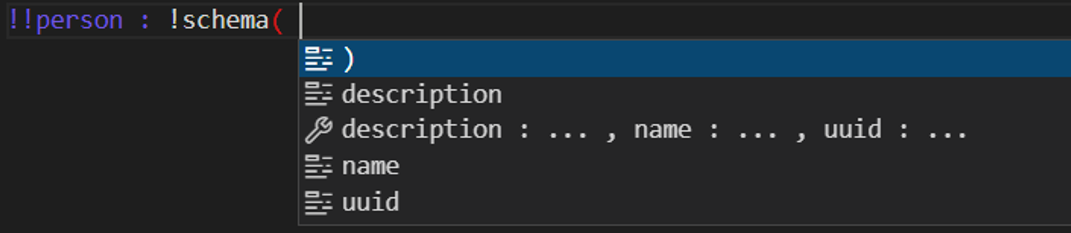
\includegraphics[width=10cm]{assets/figures/snippet-suggestion.png}
    \end{center}
    \caption[Suggestion d'un snippet]{\label{snippet-suggestion} Suggestion d'un snippet}
\end{figure}

%TODO : résultat

Il est possible de passer à la case suivante à l'aide de la touche tab. %case..
Cependant il est nécessaire de proposer ces suggestions au bon moment. La solution envisagée et de vérifier que le token du type possédant
ces propriétés ce trouve dans les candidats du moteur et qu'il ne s'agit pas de schéma % TODO

C'est un mécanisme intéressant, mais fortement lié à l'application


\subsection{Triggers}
L'éditeur va trigger automatiquement l'autocomplétions en appelant le provider lorsque l'on saisit plusieurs caractères. Il aussi possible de l'activer manuellement en exécutant la commande "ctrl + space".
On peut aussi ajouter au provider des symboles qui vont trigger son activation. Les symboles espace " " et de retour à la ligne (\\rn) ont été définis comme triggers, car cela semble assez naturel dans ce langage.
Cependant il ne s'agit que d'une appréciation personnelle.

%TODO :
No suggestion :
quand un espace précède un nouveau mot alors c'est simple pour le placer
quand il est colé c'est + compliqué. Il faut calculer la position du début et de fin du nouveau mot car VS Code peut trigger l'autocomplete n'importe quand et du coup
avec du texte colé il peut pas savoir à partir de ou le texte en train d'etre ecrit est un mot du lnagage...mais utilité de faire ça ???

%TODO : quick-suggest-setting (par défaut ?) : https://github.com/microsoft/vscode/issues/101333}

\subsection{Candidats}\label{candidates}

%Il est nécessair d'implémenter une fonction pour convertir la positon actuelle du curseur en la position du prochain token attendu.
%Pour être transmis à la fonction "collectCandidates(tokenIndex)". %todo

Il est nécessaire d'implémenter une fonction pour trouver l'indice du prochain candidat.

Actuellement ce qu'on veut c'est le prochain token possible après donc il s'agira % TODO

La documentation du projet indique bien que ce n'est pas un problème trivial à résoudre.
Un point important est de savoir si l'on tient compte ou non des espaces vides dans la grammaire.

Sans les espaces, il est difficile de gérer certains cas particuliers % TODO montrer des exemples

Actuellement pour connaitre l'indice du ou des prochains candidats, on récupère le flux des tokens (tokenStream) trouvé lors du parsing.
Puis, on récupère dans un tableau chaque token individuellement (y compris les espaces).

Cependant lorsque l'utilisateur écrit et que cela trigger l'autocomplétion, le texte parsé est souvent incorrect, car le dernier élément saisi n'est pas encore complet.

Grâce à la taille du tableau et en se basant sur les erreurs qui ont été générées, on peut déduire l'indice d'un ou des prochains tokens que l'on peut afficher.

\subsubsection{Index du candidat}
L'indexation est gérée de deux manières différentes. En fonction de la prise en compte de l'espace ou non.

\begin{figure}[!h]
    \begin{center}
        \frame{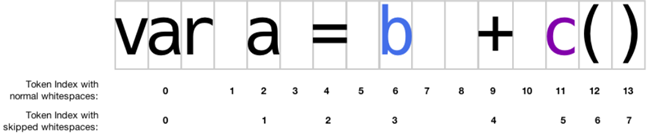
\includegraphics[width=14cm]{assets/figures/candidat-index.png}}
    \end{center}
    \caption[Indexation des candidats]{\label{candidat-index} Indexation des candidats}
\end{figure}

Cela va dépendre si on décide d'ignorer ou non les espaces dans la grammaire g4.
Les développeurs de c3 recommandent de ne pas ignorer les espaces. Car cela permet de gérer plus de cas particuliers.

\subsection{Mécanisme automatique}
VS Code va automatiquement filtrer les suggestions pendant la saisie à l'aide d'un algorithme de fuzzing search.
Pour rappel le fuzzy search (ou recherche approximative) permet de trouver une chaine de caractère en fournissant une chaine qui n'a besoin d'avoir une correspondance exacte
avec le texte que l'on cherche.

Par défaut la complétion proposée par VS Code porte sur les symboles déjà existants dans le code.
Ce type de complétion est nommé "word based completion" dans VS Code.

\section{Outline view}

La outline view est une représentation de la structure du fichier actuellement ouvert par l'éditeur.
On appelle généralement cette structure le "document outlining" ou "code outlining".

% https://code.visualstudio.com/api/references/vscode-api
% https://code.visualstudio.com/api/references/vscode-api#DocumentSymbol
% https://microsoft.github.io/language-server-protocol/specifications/lsp/3.17/specification/
En analysant les spécifications LSP ou le DocumentSymbolProvider de l'api VS Code, on constate que l'outline peut être représenté sous deux formes :

\begin{itemize}
    \item SymbolInformation qui est une flat list de tous les symboles trouvés dans un document. Dans ce cas, ni le range de localisation du symbole ni le nom du conteneur du symbole ne doivent être utilisés pour déduire une hiérarchie.
    \item DocumentSymbol qui est une hiérarchie de symboles trouvés dans un document texte donné
\end{itemize}
%TODO : citation ?

la structure peut être donc représenté de manière hiérarchique ou non (seulement être listés).

%TODO Lien

Un élément de l'outline (noeud) représente un élément unique du texte ou une structure.

On a accès à cette représentation dans le sidebar gauche par défaut.

%TODO : picture
\begin{figure}[!h]
    \begin{center}
        \frame{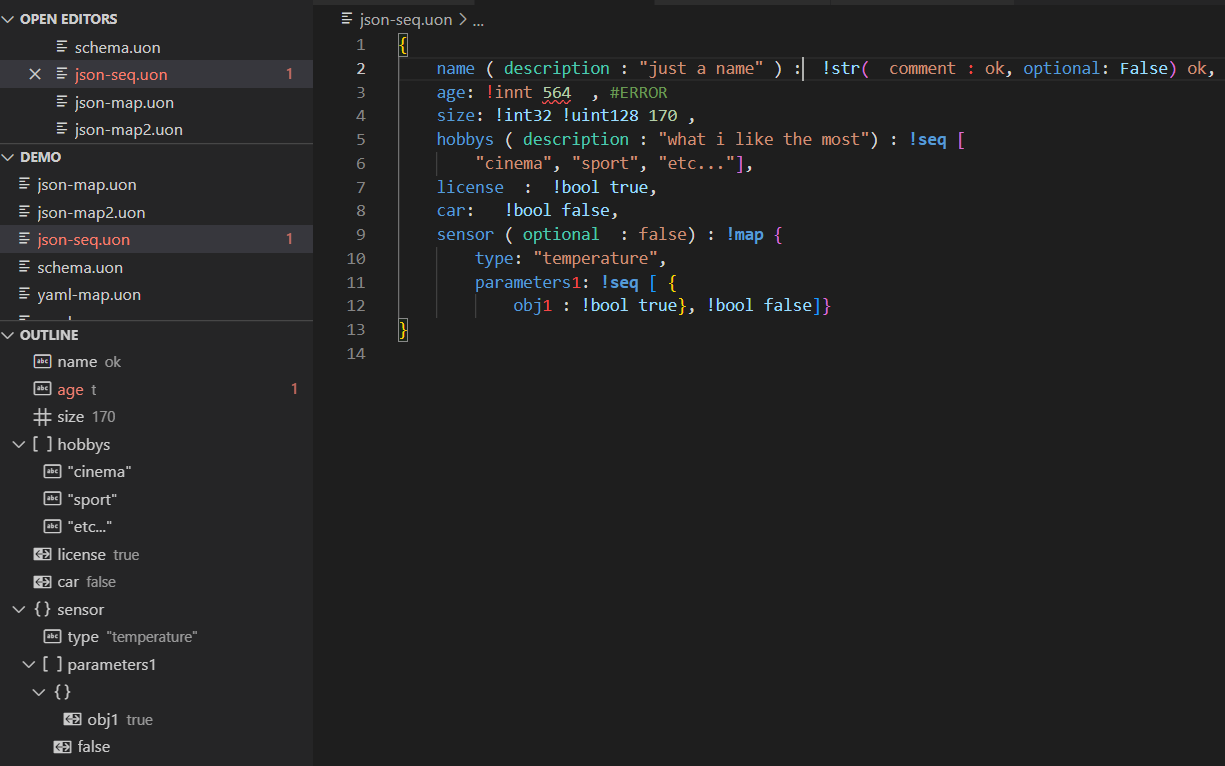
\includegraphics[width=14cm]{assets/figures/outline-view-sidebar.PNG}}
    \end{center}
    \caption[outline-view-sidebar]{\label{outline-view-sidebar} outline-view-sidebar}
\end{figure}

ou depuis la barre de recherche en saisissant la commande "CTRL + SHIFT + o" :

%TODO : picture
\begin{figure}[!h]
    \begin{center}
        \frame{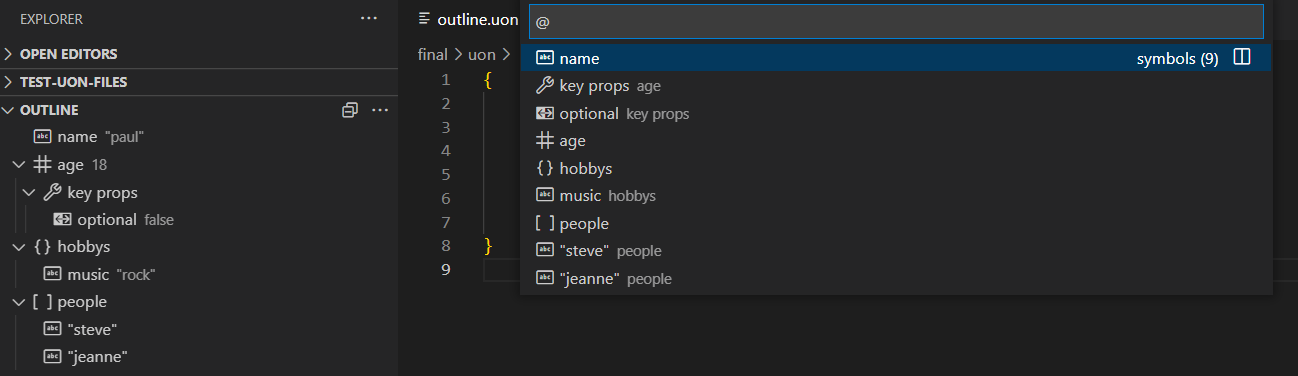
\includegraphics[width=14cm]{assets/figures/outline-view-searchbar.PNG}}
    \end{center}
    \caption[outline-view-searchbar]{\label{outline-view-searchbar} outline-view-searchbar}
\end{figure}

Il est possible obtenir la structure d'un fichier en analysant manuellement le texte (par exemple ligne par ligne).
Mais cette approche n'est pas optimale et il serait difficile de représenter la structure hiérarchique du document à l'aide de regex par exemple,
comme mentionné au point : % TODO

Nous allons donc utiliser notre parser.

Le résulat du résultat est un "parse tree" (aussi nommé CST) qui est une représentation concrète de notre input. Le parse tree contient toutes les infomrations et beaucoup d'entre elles ne nous intéressent pas.
Typiquement les informations grammaticales et structurelles.
\begin{figure}[!h]
    \begin{center}
        \frame{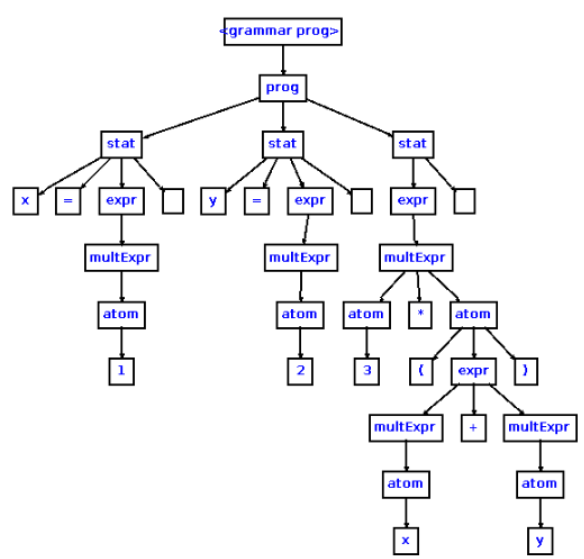
\includegraphics[width=10cm]{assets/figures/parse-tree.PNG}}
    \end{center}
    \caption[UON parse tree]{\label{parse-tree} UON parse tree}
\end{figure}

C'est pourquoi il faut pouvoir le parcourir pour en extraire un AST.
Un AST est une représentation abstraite de notre input. Il ne contient généralement que les informations les plus pertinentes.

\begin{figure}[!h]
    \begin{center}
        \frame{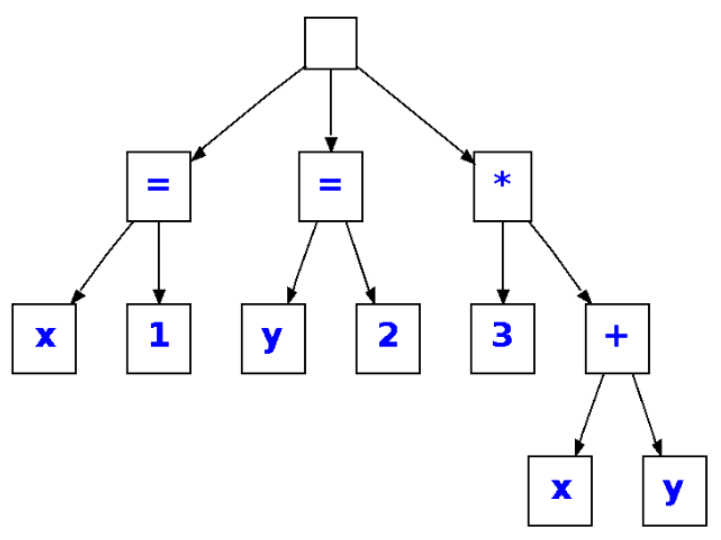
\includegraphics[width=10cm]{assets/figures/ast.PNG}}
    \end{center}
    \caption[UON AST]{\label{ast} UON AST}
\end{figure}
%TODO : Images non contractuelles

Donc pour le générer on va vouloir récupérer uniquement ces informations pendant le parcours.

Pour parcourir un arbre, deux approches sont possibles : Le pattern Listener ou Visitor.
La première consiste à écouter les types de noeuds traversés qui nous intéressent. Le problème et que cette approche ne nous permet pas de manipuler un objet en cours de route ni gérer le flux d'exécution.
Car il n'est pas possible de communiquer entre les noeuds. Cela peut être tout de même utile si l'on veut afficher la structure de l'arbre dans un terminal par exemple.

Contrairement à la seconde approche, qui nous permet de gérer ces deux cas. Et c'est donc tout naturellement que cette solution a été privilégiée.

Cependant on ne va pas d'abord créer un AST puis construire la outline view à l'aide de celui-ci.
Nous allors directement construire l'outline view à la volé, pendant le parcours du parse tree. L'outline view sera une représentation directe de notre AST.

L'arbre sera donc un objet VS Code de type \href{https://code.visualstudio.com/api/references/vscode-api#DocumentSymbol}{DocumentSymbol}.

Il y a quelques points intéressants à commenter concernant cet objet.

La variable "children" qui nous permet d'avoir des encapsulations d'objets "DocumentSymol".

Un noeud doit être représenté par un "Symbolkind" % https://vshaxe.github.io/vscode-extern/vscode/SymbolKind.html
Nous sommes donc limités sur la représentation et devons faire les ajustements nécessaires.

Il y a deux paramètres de ranges à fournir à la création de l'objet : une qui contient leur définition et une qui pointe vers leur plage la plus intéressante, par exemple la plage d'un identifiant.

Le premier se veut plus global que le second.
Dans notre cas les deux peuvent représenter la même chose et représenter la range du token affiché dans l'éditeur.

% https://stackoverflow.com/questions/55846146/make-vs-code-parse-and-display-the-structure-of-a-new-language-to-the-outline-re/63060797#63060797
%The range is the definition range (the whole definition of your symbol, e.g. for a typescript class, it starts at
%the keyword class and ends with the closing }) and the selectionRange is often only the symbol's token range
%(but according to the specification, it can also include the doc comment block and the visibility modifiers, it is the implementor's choice).

Lors de la génération des fichiers ANTLR, il est indiqué de générer également un fichier visiteur "UONVisitor" en précisant le tag "- visitor".

Cela va nous créer un fichier qui contiendra une interface définissant une fonction pour chaque type de noeud de note parseur et retournera un résultat de type générique.
Chacune de ses fonctions prend comme paramètre son contexte.

%Cette interface étends la classe \href{https://www.antlr.org/api/Java/org/antlr/v4/runtime/tree/ParseTreeVisitor.html}{ParseTreeVisitor} de ANTLR qui gère le méchanisme de parcours et d'aggrégation des résulats.

La classe UonASTVisitor implémente cette interface et étend la classe \href{https://www.antlr.org/api/Java/org/antlr/v4/runtime/tree/AbstractParseTreeVisitor.html}{AbstractParseTreeVisitor}
pour obtenir le comportement par défaut du pattern visitor.

On doit donner le "parse tree" créé par le parser à la fonction d'entrée \emph{visit} de notre visitor. % const ast = uonASTVisitor.visit(tree);

L'intérêt d'utiliser le pattern Visitor est de pouvoir retourner un élément à chaque étape du parcours.
De plus note classe \emph{UONVisitor} étant générique, c'est ce qui nous permet de manipuler un objet VS code.

%TODO : raison ?
%La classe surchargée est de type "any" car pendant le parcours un élément peu être de deux natures différentes (Une valeur/terminal ou une strucutre Vscode).


\subsection{visitChildren}
%Des fonctions de la classe AbstractParseTreeVisitor ont été surchargé pour adapter le comportement à notre situation.

La fonction \emph{visitChildren} est la suivante :

\begin{lstlisting}
1.    visitChildren(node) {
2.        let result : any = this.defaultResult();
3.        let n = node.childCount;
4.        for (let i = 0; i < n; i++) {
5.            if (!this.shouldVisitNextChild(node, result)) {
6.                break;
7.            }
8.            let c = node.getChild(i);
9.            let childResult = c.accept(this);
10.            result = this.aggregateResult(result, childResult);
12.        }
13.        return result;
14.    }
\end{lstlisting}

Le résultat par défaut est une liste vide. Lors du parcours de la remontée dans un noeud parent, nous allons rassembler les enfants dans une liste.

Pourquoi ne pas manipuler directement un objet \emph{DocumentSymbol} au lieu d'une liste ?
Tout simplement, car sinon on aurait du le faire dans la fonction d'agrégation et l'on préféra ici déléguer la logique dans le noeud parent concerné
qui pourra utiliser les valeurs récupérer pour construire l'information voulue.

C'est un choix d'implémentation pour faciliter la construction d'un objet \emph{DocumentSymbol}.

\subsection{Parcours}
Le parcours est effectué selon un algorithme de parcours en profondeur (DFS).

Pour rappel un parcours DFS est effectué dans l'ordre affiché à la figure \ref*{Algorithme de parcours en profondeur (DFS)}

\begin{figure}[!h]
    \begin{center}
        \frame{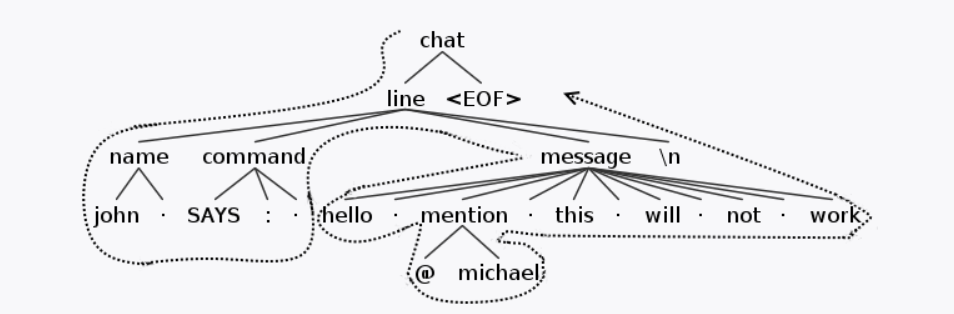
\includegraphics[width=10cm]{assets/figures/DFS.PNG}}
    \end{center}
    \caption[Algorithme de parcours en profondeur (DFS)]{\label{Algorithme de parcours en profondeur (DFS)} Algorithme de parcours en profondeur (DFS)}
\end{figure}

Ce qui est agréable en utilisant cet algorithme et qu'il nous permet de commencer à construire l'information à partir des noeuds terminaux
de l'arbre et de remonter naturellement au parent le plus proche.

Un parent va pouvoir obtenir la liste des enfants dans un ordre que l'on s'attendrait à recevoir.
Cela rend la manipulation dans un parent plus simple concernant des modifications que l'on voudrait effectuer pour représenter ces informations
dans un objet de type \emph{DocumentSymbol}.

\subsection{La position}

Généralement un noeud nous permet de nous rediriger sur l'élément du fichier lorsqu'on le sélectionne depuis la sidebar ou depuis la search bar. %todo reference
Il faut donc pouvoir être capable de récupérer la position d'un élément du fichier.

Heursement on peut récupérer cette information lors d'un parcours d'un noeud terminal du parse tree.
Il suffit d'observer le token associé au symbole de ce noeud et plus particulièrement les
propriétés \emph{line} et \emph{charPositionInLine} (qui est la position que l'on qualifierait de "colonne")
Il faut toutefois juste corriger la position de la ligne en lui soustraient une valeur de 1 car l'indice d'une ligne commence à 0 sur VS Code et 1 pour ANLTR % TODO

\subsection{Résultat}
L'aspect visuel de l'outline view à été conçu pour ressembler à celle de JSON et de YAML.
Suivant cet exemple de code UON basique :

\begin{lstlisting}
    {
        name : "paul",
        age: 18,
        hobbys: {
            music: "rock"
        },
        parents : ["steve", "jeanne"]
    }
\end{lstlisting}

Nous obtiendrons l'outline suivant :

% capture
\begin{figure}[!h]
    \begin{center}
        \frame{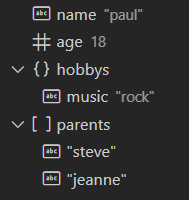
\includegraphics[width=6cm]{assets/figures/uon-payload-outline-without-properties.PNG}}
    \end{center}
    \caption[Outline UON sans propriétés]{\label{uon-payload-outline-without-properties} Outline UON sans propriétés}
\end{figure}

Mais UON prenons en compte également les propriétés, il a été jugé pertinents de les rajouter dans la outline.
Pour ne pas changer la structure et ne pas surcharger l'arbre,
nous rajoutons simplement les propriétés des clés et des types comme enfant de l'attribut parent du noeud de l'outline.

Par exemple, si nous rajoutons des propriétés à la clé est un type :
\begin{lstlisting}
    {
        name : "paul",
        age(optional : false): !int( comment : "a comment") 18,
        hobbys: {
            music: "rock"
        },
        parents : ["steve", "jeanne"]
    }
\end{lstlisting}

Nous obtiendrons l'outline suivante :

%capture
\begin{figure}[!h]
    \begin{center}
        \frame{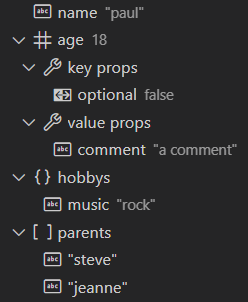
\includegraphics[width=6cm]{assets/figures/uon-payload-outline-with-properties.PNG}}
    \end{center}
    \caption[Outline UON avec propriétés]{\label{uon-payload-outline-with-properties} Outline UON avec propriétés}
\end{figure}

La représentation d'un schéma de validation est légèrement différente :

\begin{lstlisting}
    !!mySensor: !schema ( description : "provide great infos", name : ok) {
        name : !str,
        power( optional : true) : !int( min : 5, max : 50)
    }
\end{lstlisting}

Dans un fichier de validation, on ne peut avoir comme valeur uniquement des types ayant ou non des propriétés. Ce sont ces éléments qui nous intéressent le plus.
Donc on a plus de proprités "value props", mais on liste ces propriétés directement comme enfant de l'objet. Cela pour gagner en visibilité.

Nous aurons donc l'outline suivante :

\begin{figure}[!h]
    \begin{center}
        \frame{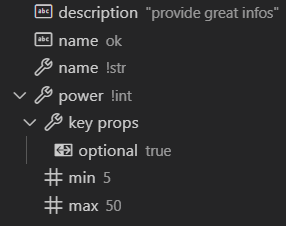
\includegraphics[width=6cm]{assets/figures/uon-schema-outline.PNG}}
    \end{center}
    \caption[Outline d'un schéma]{\label{uon-schema-outline} Outline d'un schéma}
\end{figure}

\section{Info on Hover}

C'est une fonctionnalité assez triviale qui consiste à afficher une explication lorsque l'on passe le curseur sur un élément.
Cela consiste à aller chercher dans un dictionnaire si la valeur sélectionnée est bien une clé du dictionnaire et de récupérer la valeur si c'est bien le cas.

Ce dictionnaire est un fichier.json qui est importé dans le fichier \emph{extension.js}.

Il est nécessaire de rajouter la ligne \emph{"resolveJsonModule": true} dans le fichier tsconfig.json pour autoriser ce type d'import.

Même si son implémentation est relativement simple, il n'en reste pas moins un élément fortement utile et pouvant être étendu par la suite.
Le code est déjà réutilisé pour fournir la documentation des types lors des suggestions de complétions  % \ref{}

\section{Lint}
%On affiche les erreurs trouvé avec antlr -> avantages positions
%Les erreurs sont liés au placement des tokens (manque un éléments du langages, mauvais token ou leur "ortographe").
%Message trop technique. mais ok pour voir d'ou viens la faute.


Un Linter est un outil d'analyse de code qui permet de détecter les erreurs et les problèmes de syntaxe.

Il est donc nécessaire de pouvoir exploiter correctement les erreurs.

Il est possible de créer un listener qui aura pour rôle d'observer les erreurs lors du parsing avec ANLTR.
Pour cela il faut créer une classe qui implémente l'interface "ANTLRErrorListener" et attribuer ce listener à notre parser
avec la commande :
%#parser.addErrorListener(errorListener);

Cette interface définit la fonction \emph{syntaxError}.

Cette fonction sera trigger comme sans nom l'indique lors d'une erreur de syntaxe.
Une erreur de syntaxe peut survenir quand un élément et mal orthographié ou manquant.

Il est bien de rappeler que certaines erreurs de syntaxes sont plus graves que d'autres.
Même si ANTLR propose des solutions pour se récupérer d'un processus de parsing défectueux, il reste limité et ne peut pas faire de miracle.

Elle contient des paramètres intéressants à exploiter pour informer l'utilisateur.

Sa définition est la suivante :
\begin{lstlisting}
    syntaxError?: <T extends TSymbol>(recognizer: Recognizer<T, any>, offendingSymbol: T | undefined, line: number, charPositionInLine: number, msg: string, e: RecognitionException | undefined) => void;
\end{lstlisting}

%Upon syntax error, notify any interested parties.
%This is not how to recover from errors or compute error messages.
%ANTLRErrorStrategy specifies how to recover from syntax errors and how to compute error messages.
%This listener's job is simply to emit a computed message, though it has enough information to create its own message in many cases.

Comme pour la outline %\ref*{} ,
Il est possible de récupérer la position du token. Il suffit de récupérer les valeurs des propriétés \emph{line} et \emph{charPositionInLine}.
Il s'agira ici d'un token qui a posé problème et l'on voudra afficher à son emplacement l'indication visuelle (soulignement ondulé rouge) ainsi que le message d'erreur associé, lorsque l'utilisateur passe
sa souris dessus.

Le message d'erreur peut-être récupéré à partir de la propriété \emph{msg}. Même s'il est davantage destiné au debuggage.
Les messages restent relativement simples. Ils indiquent à l'utilisateur quel token pose problème et quels sont les caractères qui pourrait y être substituer.

Pour afficher ces informations sur l'éditeur, il faut utiliser un objet VS Code de type \emph{DiagnosticCollection}.

Elle peut afficher une liste d'erreur.

On va garder en mémoire cette liste dans la classe que l'on mettra à jour à chaque fois que le listener détecte une erreur.
Et on actualisera à chaque fois l'objet \emph{DiagnosticCollection} avec cette liste.

Cependant, le parser ne pas se rendre compte si ce n'est pas plutôt le token précédent qui pourrait amener à une erreur.
Cela ne prend non plus pas en compte ce qu'il vient après et donc remplacer un token par un de ceux proposés peut se se révélé contre-productif.
% TODO

\subsection{Suggestion}
Certains messages d'erreurs nous informes parfois des tokens qui devrait se situer à la place de celui qui a causé l'erreur.
Une idée serait donc de pouvoir remplacer ce token erronées par ceux suggérés.
Le problème est que cette information ne se trouve pas sous forme textuelle.
Il faudrait donc pouvoir analyser les fichiers de stratégie et les modifier pour en récupérer la liste des tokens....

% TODO surcharger des méthodes pour pouvoir être notifié des tokens manquant

\subsection{Quick fick}

Actuellement il y a un seul quick fix qui a été implémenté, et cela à titre de découverte.

Ce quickfix permet de supprimer le token qui pose problème en se basant sur les ranges fourni lors de la création d'un objet Diagnostic depuis le listener.

À l'heure actuelle , il n'y a pas encore de suggestions. L'idée serait de pouvoir proposer un ou plusieurs tokens qui aurait du sens pour remplacer celui qui pose problème.
Et l'idéal serait de prendre en compte le texte venant après le curseur. % TODO

\section{Fonctionnalités triviales}
Il s'agit de fonctionnalités couramment disponibles dans un support de langage. Leur implémentation est relativement simple et rapide et n'a donc pas été mentionnée dans le cahier des charges.
Les suivantes ont été implémentées :

% TODO : fichier

\textbf{Comment}
\begin{itemize}
    \item Il est possible de commenter du code sous forme de ligne.
    \item Il est possible de commenter et décommenter du code (Toggling)
\end{itemize}

\textbf{Symbol pairs}
\begin{itemize}
    \item Il est possible de faire la correspondance pour certaines paires de symboles à l'aide d'une indication visuelle. (Matching)
    \item Certains symboles du langage doivent être automatiquement complétés si l'utilisateur saisit le premier élément de celle-ci. (Autoclosing)
\end{itemize}

\textbf{Code folding}
\begin{itemize}
    \item Cacher un bloc de code sur une ligne en fonction de son niveau d'indentation.
\end{itemize}

% TODO
% Couplage de fonctionnalité - logique
% Info on hover - autocompletion
% lint - code outline

\chapter{Planning}

% TODO : Ajouter discussion de l'avancée du travail. Êtes-vous à jour ? Avez-vous pris du retard ?
% TODO : Des implémentations pas compliqué mais peu de documentation sur antlrts dans le cadre d'une extension + faut trouver comment faire en testant parfois
% TODO :
%    Difficulté :
%    Regrouper toutes les sources.
%    Grand projet personnel....
%    Analyse des resultat

\subsection{Diagramme de gantt}
Voici le diagramme de Gantt pour ce projet.
Ce diagramme sera potentiellement mis à jour durant ce semestre du fait que certaines tâches ne sont pas connues à l'avance et pour réorganiser des taches si besoin.

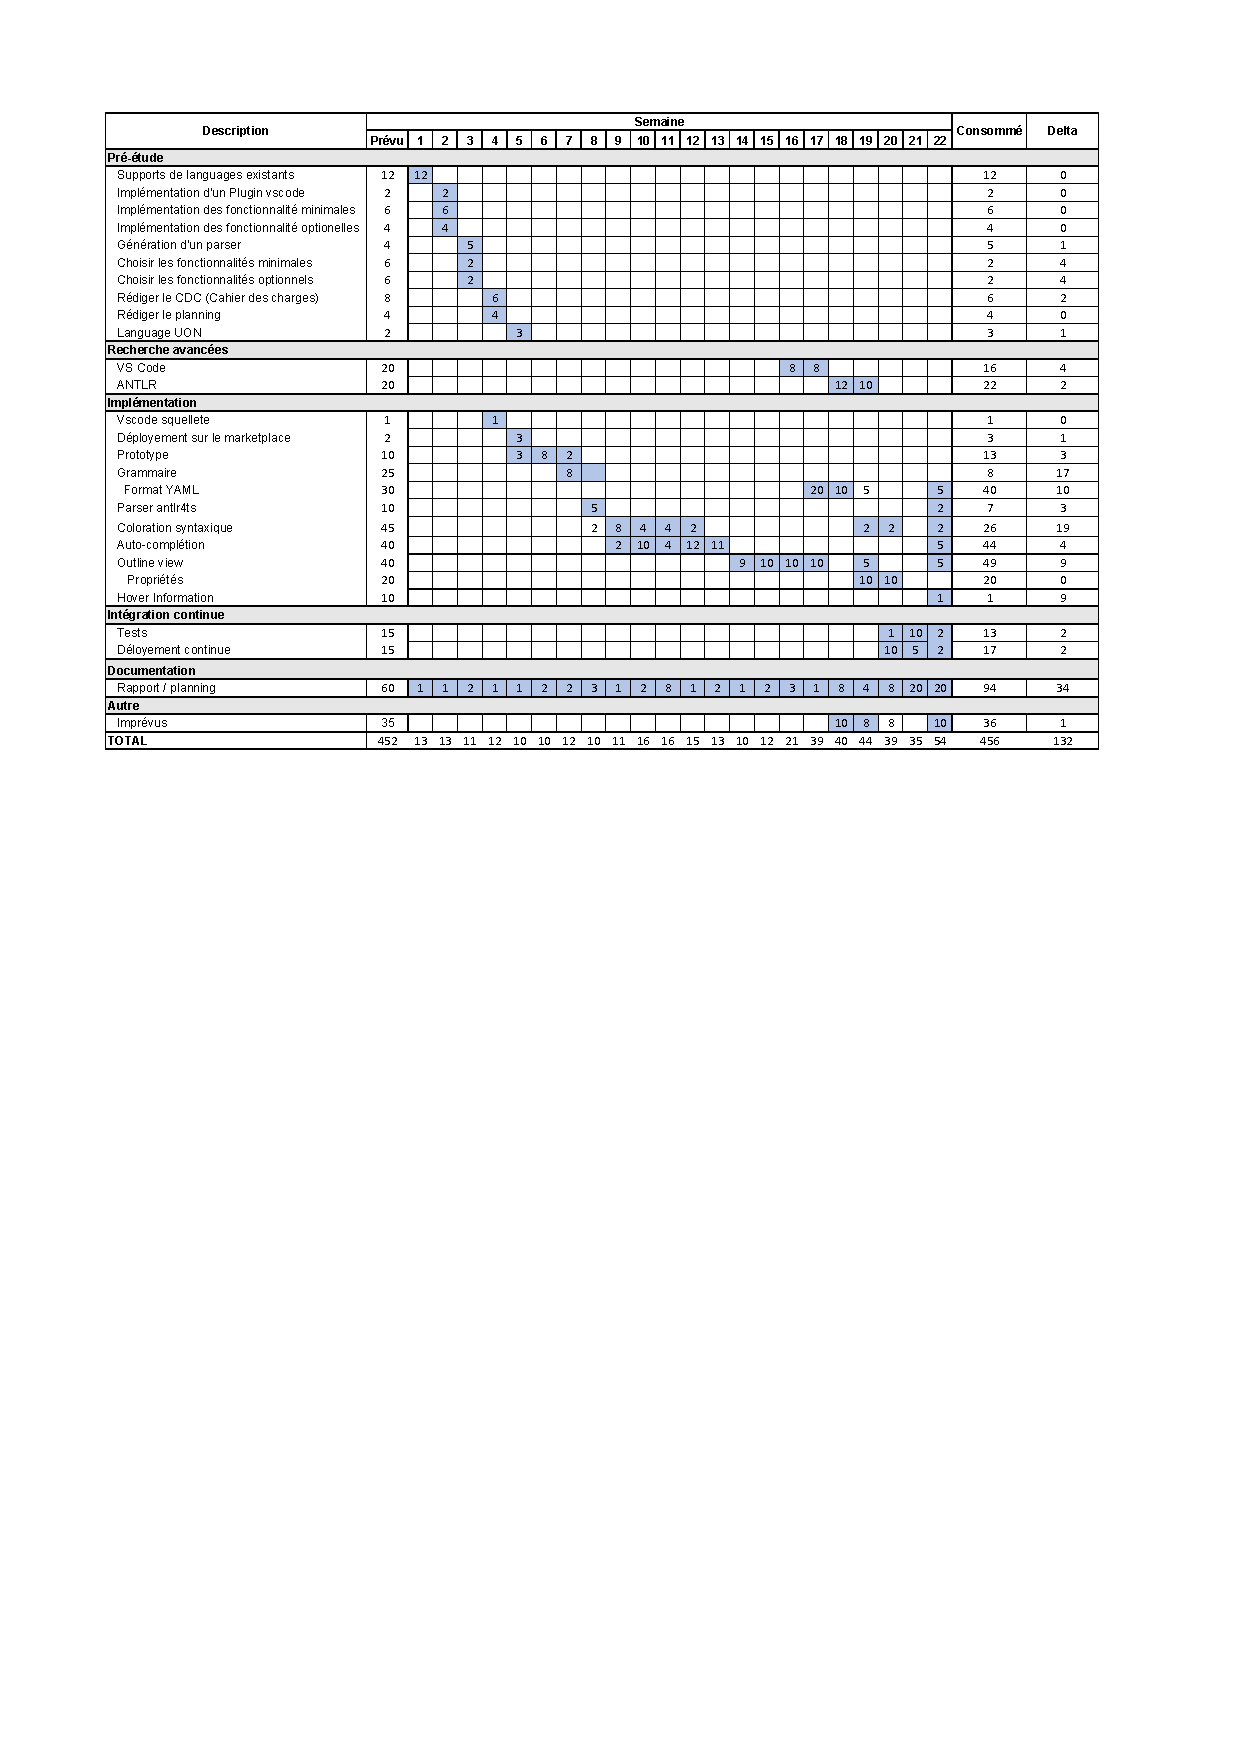
\includepdf[page=1]{assets/planning/gantt.pdf}


\chapter{Conclusion}

\section{Difficultés rencontrés}

\section{Amélioration possible}


% TODO

% what should be included in a conclusion ?
% Restate your thesis.
% Synthesize or summarize your major points.
% Make the context of your argument clear.


Travailler sur ce projet s'est révélé être très intéressant.

%L'objectif de ce travail de bachelor est de pouvoir avoir à disposition dans l'éditeur, les éléments de base pour
%Sans devoir consulter la documentation

Il a fallu découvrir et analyser un nouveau langage.
Définir quelles sont les fonctionnalités à implémenter dans un éditeur pouvant s'avérer utile comme support pour ce langage.

Découvrir les technologies permettant leur implémentation et ensuite pouvoir les utiliser en sein de notre application. % fonctionnalité cohérente entre elles


%TODO : déplacer
%Il a été mentionner à plusieurs reprises qu'un parser est un élément pouvant nous faire aboutir à notre but.
%Heursement pour nous, des outils existent pour en générer un depuis une grammaire, nous faisant gagner un temps de développement énorme.
% De plus avec cette approche, cela nous permet de travailler sur la grammaire en même temps que les fonctionnalités à implémenter.

Nous avons vu qu'il est possible de s'aider d'outils déjà existants et que cela peut, si bien utiliser, accélérer grandement la mise en place d'un support de langage.

ANTLR s'est avéré être une composante dominante du projet. De plus sa gestion des erreurs permet d'avoir une meilleure tolérance concernant les erreurs
qui sont fréquentes dans un éditeur.

L'outil de complétion c3, qui peut-être utilisé avec un parseur ANTLR a aussi été une très bonne découverte\dots

% TODO : Déplacer
%Nous avons vu est pu classifier les fonctionnalités dans deux catégories : Declarative et Programmatic features
%La première est fortement couplé à l'editeur. Pour la seconde nous avons choisi l'approche consistant à utiliser l'api de vscode.
%Mais cette api étant standardisé avec la norme LSP.
%Déplacer ces fonctionnalités en sein d'un langage serveur est possible

%% Les points d'améliorations : LSP
%% Avoir une notion de scope / schéma de validation interne si possible



%Implémenter du support nous oblige à analyser un langage en profondeur\dots

%Le support d'un langage est un sujet vaste et nous n'avons vu qu'une partie de ce qui est possible de faire.

%C'est aussi un sujet qui est très libre


Pour pouvoir fournir du support pour un langage, on est obligé de connaitre la grammaire sur laquelle ces fonctionnalités porteront.
Heursement pour nous nous avons pu reprendre une implémentation existante que nous avons adaptée pour couvrir nos besoins.

Les éléments qui ont requis le plus de travail ont été la complétion.
Car même si le moteur est extrêmement puissant et qu'il convient très bien pour notre utilisation. Il reste toutefois important de comprendre son fonctionnement et que c'est un outil pouvant s'avérer complexe.

Adapter la grammaire a été un challenge ANTLR et différent de Lark, la complétion nécessite aussi d'adapter la grammaire.

%La outline ?
%La subtilité concernant les captures regex dans la grammaires

Nous avons fait le choix de travailler uniquement dans un environnement VS Code mais fournissant toutes les clés pour des extensibilités futures

VS Code est un environnement riche et complexe, mais qui est extrêmement bien documenter et agréable à utiliser.
Il est toutefois parfois même difficile de savoir ce que peut faire cet éditeur par défaut ou non.

De plus chaque langage ayant ses spécifiés, les besoins peuvent variées les uns des autres.
Les mêmes fonctionnalités entre deux langages peuvent avoir des comportements relativement différents.

L'avantage d'avoir travaillé sur un langage de sérialisation comme UON est que cela est relativement moins complexe à gérer qu'un langage de programmation.
C'est une bonne porte d'entrée ...
Cela nous oblige à découvrir et prendre conscience ce qu'il est possible de faire plus généralement.

Mais UON est aussi plus complexe que ces concurrents sur plein de points.
Ce qu'il fait qu'il reste encore des améliorations possibles

Lors de la réalisation de ce Travail de bachelor, nous avons mis on place des mécanismes

Un point contraignant lorsque l'on développe un support de langage, et que la grammaire est intrinsèquement liée à certaines fonctionnalités.
Un changement peut avoir des répercussions sur l'ensemble de celles-ci\dots


%% \vfil
%% \hspace{8cm}\makeatletter\@author\makeatother\par
%% \hspace{8cm}\begin{minipage}{5cm}
%%if
% Place pour signature numérique
%%\printsignature
%%fi
%% \end{minipage}
%% \clearpage

%% \let\cleardoublepage\clearpage
%% \backmatter

%% TODO : Ne fonctionne pas !!!
\label{glossaire}
\printnoidxglossary
\addcontentsline{toc}{chapter}{Glossaire}

\textbf{TODO : Ajouter dans la Bibliographie https://www.regular-expressions.info/anchors.html}
\printbibliography
\addcontentsline{toc}{chapter}{Bibliographie}

%% \label{index}
%% \printindex

\end{document}
